\documentclass[12pt,letterpaper]{article}
\usepackage[utf8]{inputenc}
\usepackage{graphicx}
\usepackage{geometry}
\geometry{
    top=2.5cm,
    bottom=2.5cm,
    left=3cm,
    right=3cm
}
\usepackage{setspace}
\usepackage{tabularx}
\usepackage{tocloft}
\usepackage{amsmath,amssymb}

% Configuración de nombres en español e imágenes
\graphicspath{{docs/}{./}}
\renewcommand{\figurename}{Figura}
\renewcommand{\tablename}{Tabla}
\renewcommand{\contentsname}{ÍNDICE GENERAL}

% Configuración del Índice y Numeración
\renewcommand{\cftsecleader}{\cftdotfill{\cftdotsep}}

\begin{document}

% ==========================================
\usepackage{tocloft}
\usepackage{amsmath,amssymb}

% Configuración de nombres en español e imágenes
\graphicspath{{docs/}{./}}
\renewcommand{\figurename}{Figura}
\renewcommand{\tablename}{Tabla}
\renewcommand{\contentsname}{ÍNDICE GENERAL}

% Configuración del Índice y Numeración (Ajuste de anchos para 5.10, 5.10.1, etc.)
\renewcommand{\cftsecleader}{\cftdotfill{\cftdotsep}}
\setlength{\cftsecnumwidth}{3.0em}
\setlength{\cftsubsecindent}{3.0em}
\setlength{\cftsubsecnumwidth}{3.8em}
\setlength{\cftsubsubsecindent}{6.8em}
\setlength{\cftsubsubsecnumwidth}{4.5em}
\setlength{\cftfignumwidth}{3.0em}
\setlength{\cfttabnumwidth}{3.0em}
    {\bfseries\large CARRERA: INGENIERÍA DE SISTEMAS \par}
    
    \vspace{1.5cm}
% ==========================================
% HOJA 1: PORTADA PRINCIPAL (EXTERIOR)
% ==========================================
\begin{titlepage}
    \setlength{\parskip}{0pt}
    \centering
    
    % Logo UPSA
    
\includegraphics[width=0.42\textwidth]{Figuras/UpsaLogo.png}
    
    \vspace{1.0cm}
    
    % Facultad y Carrera
    {\bfseries\large FACULTAD DE INGENIERÍA \par}
    \vspace{0.3cm}
    {\bfseries\large CARRERA: INGENIERÍA DE SISTEMAS \par}
    
    \vspace{1.0cm}
    
    % Modalidad
    {\bfseries\large MODALIDAD DE GRADUACIÓN \par}
    \vspace{0.3cm}
    {\bfseries\large PROYECTO DE GRADO \par}
    
    \vspace{1.2cm}
    
    % Título del Proyecto
    {\bfseries\Large SISTEMA DE ANÁLISIS BIOMECÁNICO DE TÉCNICAS DE JIU-JITSU BRASILEÑO MEDIANTE INTELIGENCIA ARTIFICIAL PARA LA ACADEMIA CORPO E MENTE \par}
    
    \vfill
    
    % Autor
    {\bfseries\large Santiago Borda Zambrana \par}
    
    \vspace{1.2cm}
    
    % Ciudad y Año
    {\bfseries\large Santa Cruz de la Sierra - Bolivia \par}
    \vspace{0.3cm}
    {\bfseries\large 2026 \par}

\end{titlepage}

\clearpage

% ==========================================
% HOJA 2: PORTADA INTERIOR (SEGUNDA PORTADA)
% ==========================================
\begin{titlepage}
    \setlength{\parskip}{0pt}
    \centering
    
    % Logo UPSA
    
\includegraphics[width=0.42\textwidth]{Figuras/UpsaLogo.png}
    
    \vspace{0.8cm}
    
    % Facultad y Carrera
    {\bfseries\large FACULTAD DE INGENIERÍA \par}
    \vspace{0.2cm}
    {\bfseries\large CARRERA: INGENIERÍA DE SISTEMAS \par}
    
    \vspace{0.8cm}
    
    % Modalidad
    {\bfseries\large MODALIDAD DE GRADUACIÓN \par}
    \vspace{0.2cm}
    {\bfseries\large PROYECTO DE GRADO \par}
    
    \vspace{1.0cm}
    
    % Título del Proyecto
    {\bfseries\Large SISTEMA DE ANÁLISIS BIOMECÁNICO DE TÉCNICAS DE JIU-JITSU BRASILEÑO MEDIANTE INTELIGENCIA ARTIFICIAL PARA LA ACADEMIA CORPO E MENTE \par}
    
    \vspace{0.8cm}
    
    % Grado Académico al que opta
    {\bfseries\large Proyecto de Grado para optar al título de Licenciado(a) \par}
    \vspace{0.15cm}
    {\bfseries\large en Ingeniería de Sistemas \par}
    
    \vfill
    
    % Autor y Registro
    {\bfseries\large Santiago Borda Zambrana \par}
    \vspace{0.2cm}
    {\bfseries\large Reg.: 2021210057 \par}
    
    \vspace{1.0cm}
    
    % Ciudad y Año
    {\bfseries\large Santa Cruz de la Sierra - Bolivia \par}
    \vspace{0.2cm}
    {\bfseries\large 2026 \par}

\end{titlepage}
\vspace{1.5cm}

\begin{spacing}{1.5}
Agradezco a Dios por traerme a este mundo fuerte y saludable.

A mi madre que gracias a su amor incondicional y su esfuerzo pude estudiar, gracias mami.

A mi abuela por alimentarme y tener siempre un plato de comida.

A mis tíos por sus palabras y experiencias vividas para que aprenda.

A ti P@msyta por haberme acompañado y guiado.

Al jiujitsu brasileño, por enseñarme a afrontar los miedos, seguir incluso cuando no se ve el avance, saber lidiar con la sensación de la derrota y sobre todo a no rendirme y aprender.

\vspace{1cm}
\begin{quote}
\centering
\textit{“Un cinturón negro fue un cinturón blanco que no se rindió.”}
\end{quote}
\end{spacing}

\clearpage

% ==========================================
% HOJA 5: ABSTRACT
% ==========================================
\thispagestyle{empty}
\begin{center}
    {\bfseries\large ABSTRACT \par}
\end{center}

\vspace{0.5cm}

% Tabla Superior (Título y Autor)
\noindent
\begin{tabularx}{\textwidth}{|>{\bfseries}l|X|}
    \hline
    TÍTULO & SISTEMA DE ANÁLISIS BIOMECÁNICO DE APOYO PARA JIUJITSU BRASILEÑO PARA LA ACADEMIA CORPO E MENTE \\ \hline
    AUTOR & SANTIAGO BORDA ZAMBRANA \\ \hline
\end{tabularx}

\vspace{0.8cm}

\noindent{\bfseries PROBLEMÁTICA \par}
\vspace{0.3cm}
\noindent En el aprendizaje del Brazilian Jiu-Jitsu (BJJ), los alumnos principiantes enfrentan dificultades para evaluar su rendimiento técnico de manera objetiva. Actualmente, el progreso depende casi en su totalidad de la observación directa del profesor en tiempo real, lo que genera problemas críticos: falta de atención individualizada en clases numerosas, criterios de evaluación variables según el profesor, y una retroalimentación diferida o nula si el error no es detectado en el momento.

\vspace{0.6cm}

\noindent{\bfseries OBJETIVO GENERAL \par}
\vspace{0.3cm}
\noindent Desarrollar una aplicación móvil de apoyo para la academia Corpo e Mente que permita a los alumnos grabar sus movimientos y compararlos automáticamente con los videos de referencia de sus profesores. El sistema detectará de forma exacta los fallos en las posturas del cuerpo y entregará al alumno, de manera inmediata, recomendaciones claras y explicadas paso a paso para corregir sus errores y mejorar su aprendizaje.

\vspace{0.6cm}

\noindent{\bfseries CONTENIDO \par}
\vspace{0.3cm}
\noindent El presente trabajo de investigación se ha desarrollado bajo la metodología del Proceso Unificado (UP).

\vspace{0.8cm}

% Tabla Inferior (Metadatos del Proyecto)
\noindent
\begin{tabularx}{\textwidth}{|>{\bfseries}l|X|}
    \hline
    CARRERA & Ingeniería de Sistemas \\ \hline
    GUÍA & Velasquez Suarez Nancy Yudy \\ \hline
    DESCRIPTORES & Visión artificial, estimación de pose, inteligencia artificial generativa, base de datos vectorial, arquitectura de software, aplicación web progresiva, análisis biomecánico. \\ \hline
    EMAIL & santiagobordazambrana@gmail.com \\ \hline
    FECHA & Santa Cruz de la Sierra, 2026 \\ \hline
\end{tabularx}

\clearpage
\noindent{\bfseries CONTENIDO \par}
\vspace{0.3cm}
\noindent El presente trabajo de investigación se ha desarrollado bajo la metodología del Proceso Unificado (UP), siguiendo el enfoque iterativo, incremental y evolutivo propuesto por Craig Larman.
\thispagestyle{empty}
\begin{center}
    {\bfseries\large Resumen \par}
\end{center}

\vspace{0.8cm}

\begin{spacing}{1.5}
\noindent En este documento se aborda la problemática que enfrentan los alumnos principiantes de Brazilian Jiu-Jitsu (BJJ) para evaluar su rendimiento técnico de manera objetiva y continua. Actualmente, la retroalimentación depende exclusivamente de la observación y experiencia del profesor, lo que genera evaluaciones subjetivas. Esto provoca que el alumno permanezca estancado en su progreso de aprendizaje por periodos prolongados. En respuesta a esta necesidad, se propone el desarrollo de una aplicación web progresiva (PWA) que integra inteligencia artificial y visión por computadora para analizar videos de entrenamiento.

\vspace{0.4cm}

\noindent El desarrollo del software se divide en cuatro etapas metodológicas bajo el Proceso Unificado (UP): Inicio, Elaboración, Construcción y Transición.
\end{spacing}

\clearpage

% ==========================================
% HOJA 7: ÍNDICE GENERAL (TABLA DE CONTENIDOS)
% ==========================================
\thispagestyle{empty}
\begin{spacing}{1.15}
\tableofcontents
\end{spacing}

\clearpage
\pagenumbering{arabic}
\setcounter{page}{1}

% Reconfiguración de numeración para el Capítulo I (1.1, 1.1.1, etc.)
\renewcommand{\thesection}{1.\arabic{section}}
\renewcommand{\thesubsection}{1.\arabic{section}.\arabic{subsection}}

% ==========================================
% CAPÍTULO I: DEFINICIÓN DEL PROYECTO
% ==========================================
\begin{center}
    {\bfseries\Large CAPÍTULO I: DEFINICIÓN DEL PROYECTO DE INVESTIGACIÓN \par}
\end{center}
\addcontentsline{toc}{section}{\textbf{CAPÍTULO I: DEFINICIÓN DEL PROYECTO DE INVESTIGACIÓN}}
\vspace{1cm}

\section{Definición del problema}

\subsection{Situación problemática}
En la enseñanza del Jiu-Jitsu Brasileño (BJJ) dentro de la academia \textit{Corpo e Mente}, los alumnos principiantes e intermedios enfrentan dificultades significativas para evaluar y perfeccionar su ejecución técnica de manera objetiva y continua. En el modelo tradicional, la enseñanza depende casi exclusivamente de la observación directa y presencial del profesor durante clases grupales numerosas. 

Esta dinámica genera los siguientes problemas críticos:
\begin{itemize}
    \item \textbf{Atención individualizada limitada:} En clases con alta afluencia de alumnos, el profesor no puede observar la totalidad de las repeticiones ejecutadas por cada alumno.
    \item \textbf{Retroalimentación diferida o ausente:} Si un error postural o de apalancamiento no es detectado en el instante preciso de la ejecución, el alumno tiende a automatizar patrones de movimiento incorrectos.
    \item \textbf{Evaluación subjetiva sin métricas cuantitativas:} La corrección tradicional carece de mediciones objetivas sobre ángulos articulares, alineación espinal o posición del cuerpo.
    \item \textbf{Riesgo incrementado de lesiones:} La repetición continua de técnicas con una biomecánica defectuosa expone a las articulaciones a sobrecargas y tensiones anómalas.
    \item \textbf{Progreso estancado fuera del aula:} El alumno no dispone de herramientas de autoevaluación guiadas fuera de los horarios de entrenamiento para comparar su desempeño con la técnica patrón enseñada por su profesor.
\end{itemize}

\subsection{Situación deseada}
La situación deseada consiste en implementar una solución tecnológica de apoyo para la academia \textit{Corpo e Mente} basada en una aplicación web que integre visión por computadora e inteligencia artificial generativa.

Con esta solución se logrará:
\begin{enumerate}
    \item Permitir al alumno grabar sus ejecuciones técnicas desde su dispositivo móvil en cualquier momento.
    \item Extraer automáticamente la postura corporal del alumno y compararla de forma analítica con la técnica patrón registrada por el profesor.
    \item Identificar desajustes articulares y generar reportes pedagógicos estructurados (análisis postural, riesgo de lesión y corrección paso a paso).
    \item Entregar retroalimentación objetiva, inmediata y fundamentada en literatura especializada de BJJ, acelerando la curva de aprendizaje técnico y reduciendo el riesgo de lesiones.
\end{enumerate}

\subsection{Objeto de investigación}
El objeto de investigación es el proceso de evaluación y corrección biomecánica postural de técnicas de Jiu-Jitsu Brasileño mediante visión por computadora y modelos de lenguaje orquestados bajo arquitecturas de recuperación de información.

\subsection{Alcance}

\subsection{Situación problemática}

El análisis operativo de la filial revela los siguientes indicadores críticos:
\begin{itemize}
    \item \textbf{Dependencia total del profesor:} Durante la clase de 90 minutos, con 15 alumnos y 675 repeticiones totales, el profesor dispone de 8 segundos por repetición para corregir. Esto deja más del 80\% de los errores técnicos sin retroalimentación. Fuera del aula, el alumno no tiene ninguna forma objetiva de saber si está practicando bien.
    \item \textbf{Frustración al aplicar la técnica:} El alumno que aprende solo con videos replica la forma exterior del movimiento, pero no comprende sus detalles biomecánicos. Cuando intenta ejecutar la técnica durante un combate, esta falla. La repetición del fracaso refuerza la percepción de estancamiento.
\end{itemize}
\subsubsection{Alcance Tecnológico}
\begin{itemize}
    \item \textbf{Aplicación Web y Servidor de Procesamiento:} Arquitectura cliente-servidor orientada a servicios para la captura de video, procesamiento de imágenes y almacenamiento de información.
    \item \textbf{Modelos de Inteligencia Artificial:} YOLO26x-Pose + YOLO26x-Depth para estimación de pose 3D (17 keypoints COCO), Qwen3-VL-Embedding-2B para vectorización densa de 2048 dimensiones, Gemini 2.5 Flash para síntesis pedagógica estructurada en JSON.
\end{itemize}

\subsubsection{Exclusiones}
\begin{itemize}
    \item El sistema no sustituye la evaluación presencial formal ni el criterio del maestro para la graduación de cinturones.
    \item No realiza diagnósticos médicos o clínicos fisioterapéuticos de rehabilitación.
\end{itemize}

\subsection{Justificación}

\subsubsection{Justificación Técnica y de Diseño del Producto}
\textbf{Alcance funcional:} El sistema incluye autenticación por roles (Profesor y Alumno), registro obligatorio del video semilla del profesor, carga de videos cortos (hasta 30 segundos) de ejercicios individuales (Solo Drills), detección de 17 keypoints COCO-Pose en 3D y evaluación biomecánica de 8 a 12 ángulos articulares clave, comparación cinemática con el patrón del profesor mediante DTW, generación de reportes pedagógicos en cuatro bloques (Análisis Postural, Alertas, Guía Paso a Paso y Resumen), historial de progreso del alumno, panel analítico del profesor y mantenimiento nocturno autónomo.

\subsubsection{Justificación Económica, Institucional y de Negocio}
Actualmente, el principal generador de ingresos de la sucursal anfitriona (Knockout Gym) es un modelo paquetizado de 300 Bs mensuales por acceso ilimitado, donde el Jiu-Jitsu interactúa con otras disciplinas de manera indirecta dentro de un control de accesos centralizado (administrado mediante sistemas tradicionales como Microsoft Access y lectores de huella locales). Dado que Knockout controla el flujo de caja global y Corpo e Mente no tiene injerencia en la cobranza diaria de este punto, la academia necesita consolidar un factor de valor agregado y diferenciación comercial exclusiva para justificar su permanencia, aumentar su poder de negociación frente al gimnasio y captar un mayor porcentaje de los ingresos del paquete.

Más allá de este caso de estudio local, la viabilidad económica del proyecto radica en su capacidad de Escalabilidad y Comercialización Internacional bajo un modelo de negocio de Software como Servicio (SaaS). El sistema no está diseñado como una herramienta aislada, sino como un producto empaquetado listo para ser monetizado en el mercado global de las artes marciales mediante dos vías de ingresos:

\begin{itemize}
    \item \textbf{Modelos de Licenciamiento por Volumen:} Venta de licencias anuales a academias y redes de dojos de cualquier país, parametrizadas y cobradas según la capacidad de alumnos registrados en su base de datos (Slots de usuarios).
    \item \textbf{Contratos de Soporte y Actualizaciones de Contenido:} Cobros anuales recurrentes por soporte técnico, mantenimiento y la actualización constante del catálogo de conocimientos y videotutoriales con profesores de alto rango internacional.
\end{itemize}

De este modo, el proyecto pasa de ser un gasto operativo a convertirse en un activo tecnológico de alta rentabilidad que eleva el valor de mercado de Corpo e Mente y abre una nueva línea de ingresos digitales escalables.

\newpage

\section{Objetivos}

\subsection{Objetivo General}
Desarrollar un sistema de apoyo para el análisis biomecánico de movimientos en Jiu-Jitsu Brasileño para la academia \textit{Corpo e Mente}, mediante visión por computadora e inteligencia artificial, que permita evaluar objetivamente las ejecuciones técnicas de los alumnos y proporcionar retroalimentación pedagógica estructurada en tiempo real.

\subsection{Objetivos Específicos}
\begin{enumerate}
    \item Analizar y especificar los requerimientos del sistema y casos de uso para el registro de patrones técnicos y la evaluación biomecánica.
    \item Implementar el módulo de visión por computadora para la detección y extracción de posturas corporales a partir de videos de entrenamiento.
    \item Desarrollar el algoritmo de comparación biomecánica para computar las diferencias angulares articulares entre la ejecución del alumno y la técnica patrón del profesor.
    \item Construir el motor de búsqueda semántica para recuperar información explicativa desde literatura especializada de Jiu-Jitsu Brasileño.
    \item Integrar el modelo de lenguaje generativo para elaborar reportes de retroalimentación pedagógica en análisis postural, riesgo de lesión, guía paso a paso y resumen ejecutivo.
    \item Desarrollar una interfaz web intuitiva y responsiva que permita la interacción eficiente entre profesores y alumnos.
    \item Validar la solución mediante pruebas unitarias, de integración y funcionales.
\end{enumerate}

\newpage

\section{Metodología}

\subsection{Ingeniería de Software (Proceso Unificado)}
Para el desarrollo del software se adopta la metodología del Proceso Unificado (UP), guiada por casos de uso, centrada en la arquitectura de software e iterativa e incremental. Su ciclo de vida comprende cuatro fases:

\begin{enumerate}
    \item \textbf{Fase de Inicio (Inception):} Definición de los objetivos del proyecto, delimitación del alcance y evaluación de factibilidad.
    \item \textbf{Fase de Elaboración (Elaboration):} Especificación detallada de casos de uso, diseño de la arquitectura en capas y prototipado del motor biomecánico.
    \item \textbf{Fase de Construcción (Construction):} Desarrollo iterativo de los componentes del servidor (FastAPI), modelos de inteligencia artificial (YOLO26x en Colab GPU, Qwen3-VL-Embedding-2B, Gemini 2.5 Flash), pipeline RAG (Qdrant + PostgreSQL BCNF) e interfaz web progresiva (PWA).
    \item \textbf{Fase de Transición (Transition):} Pruebas del sistema, optimización de componentes y despliegue final para la academia \textit{Corpo e Mente}.
\end{enumerate}

\subsection{Gestión del Proyecto (Scrum)}
La gestión operativa del proyecto se alinea con el marco ágil \textbf{Scrum}, organizando el trabajo en iteraciones cortas denominadas Sprints:

\begin{itemize}
    \item \textbf{Planificación Temporal y Cronograma:} El desarrollo del proyecto contempla una duración total de un (1) año, iniciando las actividades de investigación y desarrollo en febrero de 2026 y finalizando con el despliegue y validación en diciembre de 2026.
    \item \textbf{Product Backlog:} Lista priorizada de requisitos y funcionalidades del sistema.
    \item \textbf{Sprints:} Ciclos de trabajo de 2 semanas para la entrega de incrementos funcionales probados del software.
    \item \textbf{Aseguramiento de Calidad:} Desarrollo guiado por pruebas para validar el correcto funcionamiento de la lógica de negocio e interfaces.
    \item \textbf{Control de Versiones:} Gestión del código fuente mediante control de versiones y gestión de entornos de trabajo.
\end{itemize}

\clearpage

% Reconfiguración de numeración para el Capítulo II (2.1, 2.1.1, etc.)
\renewcommand{\thesection}{2.\arabic{section}}
\renewcommand{\thesubsection}{2.\arabic{section}.\arabic{subsection}}
\setcounter{section}{0}

% ==========================================
% CAPÍTULO II: MARCO INSTITUCIONAL
% ==========================================
\begin{center}
    {\bfseries\Large CAPÍTULO II: MARCO INSTITUCIONAL \par}
\end{center}
\addcontentsline{toc}{section}{\textbf{CAPÍTULO II: MARCO INSTITUCIONAL}}
\vspace{1cm}

\section{Antecedentes Institucionales}
La academia \textit{Corpo e Mente} (asociada al centro de entrenamiento \textit{KnockOut Training Center}) es una institución especializada en la enseñanza y perfeccionamiento de artes marciales y deportes de contacto, destacando principalmente en la disciplina del Jiu-Jitsu Brasileño (BJJ) y Judó. Fundada con el propósito de fomentar la disciplina física, mental y el desarrollo deportivo integral bajo la dirección técnica del maestro Humberto Tavares, la academia ofrece programas de formación orientados a practicantes de diversos niveles de experiencia, desde principiantes hasta competidores de alto rendimiento.

\begin{figure}[htbp]
    \centering
    
\includegraphics[width=0.35\textwidth]{corpo.jpeg}
    \hspace{1cm}
    
\includegraphics[width=0.35\textwidth]{KnockOut.jpg}
    \caption{Logotipos Institucionales: Academia Corpo e Mente y KnockOut Training Center}
    \label{fig:logotipos_institucionales}
\end{figure}


\section{Estructura Orgánica (Organigrama)}

La estructura organizacional que rige el funcionamiento de la academia se presenta en la Figura \ref{fig:organigrama}, detallando la jerarquía internacional de la asociación y su descentralización operativa dentro del territorio boliviano, con especial énfasis en el nodo correspondiente al objeto de estudio.

El modelo responde a una estructura mixta (lineal-funcional) que opera bajo un esquema descentralizado de matriz-filial y alianzas estratégicas de infraestructura corporativa. A continuación, se describen los niveles y componentes que integran esta estructura:

\begin{itemize}
    \item \textbf{1. Nivel Estratégico Internacional (Sede Matriz - Brasil):} Representa la máxima autoridad doctrinaria y metodológica de la escuela, liderada a nivel global por el fundador Master Humberto Tavares. Este nivel se encarga de emitir los lineamientos técnicos oficiales y validar las certificaciones internacionales de grados ante entes reguladores globales como la International Brazilian Jiu-Jitsu Federation (IBJJF). Su relación con la filial nacional es estrictamente doctrinal y de auditoría técnica, sin interferencia directa en la gestión financiera local.
    
    \item \textbf{2. Nivel de Coordinación Nacional (Corpo e Mente - Estructura Central Bolivia):} Estructura encargada de centralizar la personería de la marca en el país. Está dirigida por la Dirección General / Representante Nacional, unidad de la cual dependen las áreas funcionales de Gestión de Afiliaciones e Inscripciones (responsable del ecosistema digital en la plataforma Smoothcomp) y la Coordinación de Eventos y Selectivos (encargada de la logística de torneos inter-academias). Este nivel supervisa de manera directa la Red de Sucursales distribuidas en la ciudad de Santa Cruz de la Sierra (Sucursal UFC Gym, Sucursal 3 Pasos al Frente, Sucursal UAGRM y la célula del Programa en KnockOut).
    
    \item \textbf{3. El Gimnasio Independiente (Convenio Proveedor Externo - KnockOut Gym):} KnockOut Gym opera como un ente administrativo y legalmente independiente a Corpo e Mente. La relación institucional se define mediante una Alianza Estratégica de Tercerización de Infraestructura (Outsourcing) bajo un formato horario específico. KnockOut Gym funge como el agente de recaudación y cobro de membresías mensuales de los alumnos de Jiu-Jitsu, asumiendo el riesgo comercial del espacio y ejecutando posteriormente el desembolso económico correspondiente (por horas de clase o porcentaje acordado) hacia el cuerpo docente de la academia. KnockOut Gym no posee participación alguna en la toma de decisiones organizacionales, metodológicas o de graduaciones de Corpo e Mente, limitándose contractualmente al alquiler del espacio físico del tatami.
    
    \item \textbf{4. Estructura Operativa Interna (Célula Operativa Nocturna - Sucursal KnockOut):} Representa el alcance físico e institucional donde se acota el despliegue del sistema de software desarrollado. Debido a la naturaleza de la alianza con el gimnasio anfitrión, la operación se simplifica en una estructura lineal de turno único enfocado en el horario nocturno.
    \begin{itemize}
        \item \textbf{Profesor Encargado (Prof. Miguel Baigorria - Cinturón Negro):} Unidad responsable del desarrollo técnico, la planificación de las clases, la supervisión de la seguridad y el enlace operativo con la administración de KnockOut Gym. En el contexto del sistema BJJ Biomechanics, este puesto asume de forma exclusiva el rol de Profesor, encargándose de alimentar el catálogo de técnicas patrón, cargar videos de referencia cinemática y gestionar el repositorio semántico del motor RAG.
        \item \textbf{Alumnos y Atletas de BJJ (Turno Noche):} Usuarios finales del programa de entrenamiento nocturno. Dentro del alcance del software, asumen el rol de Alumno, interactuando con la Aplicación Web Progresiva (PWA) para registrar sus ejecuciones y recibir la retroalimentación biomecánica automatizada orientada a optimizar su curva de aprendizaje.
    \end{itemize}
\end{itemize}

\begin{figure}[htbp]
    \centering
    
\includegraphics[width=0.85\textwidth]{Organigrama.png}
    \caption{Organigrama Estructural de KnockOut Training Center}
    \label{fig:organigrama}
\end{figure}

\section{Flujo del Negocio y Análisis de Procesos}
El flujo operativo tradicional para la atención y formación de los alumnos dentro de la academia sigue una serie de pasos secuenciales desde su registro administrativo hasta el entrenamiento en el tatami.

\begin{figure}[htbp]
    \centering
    
\includegraphics[width=0.95\textwidth]{Flujo del negocio.png}
    \caption{Diagrama del Flujo del Negocio de la Academia y Detección del Cuello de Botella}
    \label{fig:flujo_negocio}
\end{figure}

El proceso operativo ilustrado en la Figura~\ref{fig:flujo_negocio} comprende las siguientes etapas:
\begin{enumerate}
    \item El alumno se dirige a la administración para solicitar información o renovar su membresía.
    \item La administración muestra el catálogo de disciplinas disponibles (BJJ, Judó).
    \item El alumno selecciona la disciplina de su preferencia (foco principal en BJJ).
    \item El alumno realiza el pago de la disciplina seleccionada en la recepción.
    \item La administración registra el pago en el sistema contable.
    \item La administración entrega el recibo o comprobante de inscripción al alumno.
    \item El alumno ingresa al área de entrenamiento y entrega el comprobante de pago al profesor asignado.
    \item El profesor imparte la clase técnica y guía el entrenamiento del alumno.
    \item \textbf{Cuello de Botella Identificado (Evaluación del Practicante):} La evaluación personalizada de posturas y ejecuciones biomecánicas por parte del profesor constituye un punto crítico de estrangulamiento. Debido al número de alumnos por clase y al tiempo limitado del entrenamiento presencial, el profesor no puede realizar una retroalimentación continua e individualizada para cada repetición técnica.
\end{enumerate}

El sistema de software propuesto viene a resolver directamente este cuello de botella, permitiendo que la evaluación técnica sea automatizada mediante visión artificial e inteligencia artificial.

El cuello de botella identificado (evaluación personalizada) es resuelto directamente por el caso de uso CU-02 (Evaluar Ejecución Biomecánica con Síntesis Pedagógica), implementado en el controlador EvaluacionController y expuesto vía POST /api/v1/alumno/evaluaciones.
\begin{enumerate}
    \item \textbf{Filtrado Topológico y Selección Articular:} Se detectan los 17 keypoints anatómicos del estándar COCO-Pose (índices 0 a 16). A partir de estos 17 puntos detectados por YOLO26x-Pose, la \texttt{CalculadoraBiomecanica} selecciona los puntos articulares relevantes y evalúa entre 8 y 12 ángulos articulares tridimensionales clave según la técnica monitoreada (codos, hombros, rodillas, caderas, tobillos y eje axial del tronco, en lados izquierdo y derecho).

    \item \textbf{Fusión Geométrica 3D (YOLO26x-Pose + YOLO26x-Depth):} Para cada keypoint 2D $(x, y)$ detectado por YOLO26x-Pose, se escala a las coordenadas del mapa de profundidad $(x_d, y_d)$ generado por YOLO26x-Depth y se extrae la componente Z métrica en metros reales:
\[
Z = \text{depth-map}[y_d, x_d]
\]
\textit{En palabras simples: esta fórmula asigna a cada articulación su profundidad en metros reales, sin necesidad de sensores RGB-D costosos.}

    \item \textbf{Traslación de Origen al Sacro:} Se toma el punto medio de las caderas (pelvis/sacro) como el origen de coordenadas $\mathbf{p}_{\text{root}} = (0,0,0)$:
\[
\mathbf{p}'_{k}(t) = \mathbf{p}_{k}(t) - \mathbf{p}_{\text{root}}(t), \quad \forall k \in \{0, \dots, 16\}
\]
\textit{En palabras simples: esta fórmula centra los 17 keypoints COCO del cuerpo tomando la cadera como punto cero.}

\section{Fundamentos Teóricos}

\subsection{Jiu-Jitsu Brasileño (BJJ) y Análisis Biomecánico Postural}
El Jiu-Jitsu Brasileño es un deporte de combate y arte marcial centrado en la lucha cuerpo a cuerpo (\textit{grappling}), donde la victoria se logra mediante el dominio de posiciones de control o la aplicación de técnicas de sometimiento (palancas articulares y estrangulamientos). La efectividad de una técnica radica en principios físicos fundamentales: aprovechamiento de palancas cinemáticas, alineación de ejes articulares, gestión del centro de masa corporal y optimización del apalancamiento mecánico.

El análisis biomecánico en el BJJ estudia el movimiento corporal y las fuerzas involucradas durante la ejecución de las técnicas. La evaluación de los ángulos articulares en puntos críticos (hombros, codos, caderas, rodillas y tobillos) permite determinar cuantitativamente si la ejecución de un alumno coincide con el patrón ideal dictado por el profesor o si presenta desviaciones que comprometan la eficacia técnica o incrementen el riesgo de lesiones.

\subsection{Estimación de Pose Corporales y Profundidad Métrica Monocular}
La estimación de pose es una rama de la visión por computadora encargada de identificar y rastrear la posición espacial de nodos articulares anatómicos (\textit{keypoints}) en fotogramas de video. Combinada con la estimación de profundidad métrica monocular, es posible reconstruir las coordenadas cinemáticas en tres dimensiones $\mathbb{R}^3 (X, Y, Z)$ en metros reales absolutos, sin necesidad de emplear cámaras físicas o sensores infrarrojos RGB-D costosos.

La fusión geométrica se realiza mediante muestreo bilineal: para cada keypoint 2D (x, y) detectado por YOLO26x-Pose, se escala a las coordenadas del mapa de profundidad (x\_d, y\_d) y se extrae la componente Z métrica: Z = depth\_map[y\_d, x\_d], expresada en metros reales. La matriz resultante es una MatrizEsqueletica de dominio con puntos Punto3D(x, y, z).

\subsection{Recuperación Aumentada por Generación (RAG)}
El pipeline RAG implementado consta de 5 etapas:
\begin{enumerate}
    \item Fragmentación semántica: ChunkerSemanticoBJJ con RecursiveCharacterTextSplitter (chunk\_size=1000, chunk\_overlap=200).
    \item Vectorización: Qwen3-VL-Embedding-2B (2048 dimensiones, normalizado).
    \item Almacenamiento vectorial: Qdrant local (colección 'bjj\_knowledge', métrica Cosine, búsqueda KNN con filtro por id\_tecnica).
    \item Persistencia relacional: PostgreSQL BCNF (tabla fuentes\_conocimiento con id\_documento para agrupar chunks).
    \item Generación: Gemini 2.5 Flash con salida JSON estricta (4 claves).
\end{enumerate}

\newpage

\section{Selección y Justificación Tecnológica}

En esta sección se describen en detalle las tecnologías seleccionadas para la implementación del sistema informático, presentando el análisis comparativo y la justificación técnica de cada elección frente a otras alternativas existentes en el mercado.

\subsection{Módulo de Visión Artificial: Suite YOLO26x-Pose + YOLO26x-Depth}

\subsubsection{Tecnología Seleccionada}
Se seleccionó la suite combinada de \textbf{YOLO26x-Pose} (detección de 17 articulaciones anatómicas COCO) y \textbf{YOLO26x-Depth} (mapa de profundidad métrica monocular en metros reales absolutos).

\subsubsection{Alternativas Consideradas}
\begin{itemize}
    \item \textbf{OpenPose / MediaPipe:} Opciones tradicionales para estimación de pose 2D/3D.
    \item \textbf{Sensores RGB-D (Kinect / Intel RealSense):} Hardware especializado que captura profundidad.
\end{itemize}

\subsubsection{Justificación de la Selección}
\begin{table}[htbp]
\centering
\small
\begin{tabularx}{\textwidth}{|>{\bfseries}l|X|X|X|}
    \hline
    Criterio & YOLO26x-Pose + Depth & MediaPipe (Google) & OpenPose \\ \hline
    Contacto Corporal & Alto desempeño en agarres y oclusión. & Falla con solapamiento de dos personas. & Bueno pero muy lento en CPU. \\ \hline
    Profundidad 3D & Profundidad métrica real $Z$ vía YOLO Depth. & Sin profundidad métrica real absoluta. & Requiere calibración compleja. \\ \hline
    Velocidad / Latencia & Inferencia sincrónica en tiempo real sobre GPU. & Muy rápida en móvil. & Latencia elevada (baja velocidad). \\ \hline
\end{tabularx}
\caption{Cuadro Comparativo de Tecnologías de Estimación de Pose y Profundidad}
\label{tab:comp_pose}
\end{table}

\textbf{YOLO26x-Pose (Ultralytics, 2026):} Detector de pose de última generación optimizado para mantener un tracking confiable bajo oclusión moderada. Extrae los 17 keypoints COCO (índices 0 a 16) en cada fotograma a 30 FPS. Posteriormente, la \texttt{CalculadoraBiomecanica} evalúa exactamente 8 ángulos articulares tridimensionales (codos, rodillas, hombros y caderas, en sus lados izquierdo y derecho) a partir de esta topología. En videos de práctica cooperativa, YOLO26x opera en modo multi-persona: detecta dos esqueletos simultáneos, y el sistema asigna el esqueleto del alumno según la posición indicada manualmente en la PWA.

En Jiu-Jitsu Brasileño, dos practicantes interactúan en contacto físico estrecho, generando oclusiones constantes de extremidades. \textbf{MediaPipe} fue descartado debido a su baja tolerancia al solapamiento corporal y pérdida de seguimiento en posiciones de suelo. \textbf{OpenPose} fue descartado por requerir un consumo excesivo de memoria y latencias altas. La combinación de \textbf{YOLO26x-Pose + YOLO26x-Depth} permite obtener coordenadas reales $(X, Y, Z)$ en metros dentro del espacio tridimensional sin requerir sensores hardware RGB-D. La inferencia de YOLO26x-Pose + YOLO26x-Depth se delega a Google Colab Pro (GPU NVIDIA T4/A100) mediante un servidor Flask expuesto por túnel Ngrok. El backend FastAPI local consume el endpoint \texttt{POST /inferir} y recibe \texttt{keypoints\_3d + frame\_base64}. Si el túnel no está disponible, el sistema usa \texttt{AdaptadorYOLO} con \texttt{MockYOLOEngine} como fallback (ver \texttt{src/infrastructure/adapters/yolo\_adapter.py}).


\subsection{Infraestructura de Inferencia GPU en la Nube: Google Colab GPU + Ngrok}

\subsubsection{Tecnología Seleccionada}
Se seleccionó un servidor de inferencia remoto alojado en **Google Colab** respaldado por procesadores GPU (NVIDIA T4 / A100), comunicado con la aplicación backend a través de un túnel seguro **Ngrok**.

\subsubsection{Alternativas Consideradas}
\begin{table}[htbp]
\centering
\footnotesize
\begin{tabularx}{\textwidth}{|>{\bfseries\raggedright\arraybackslash}X|>{\raggedright\arraybackslash}X|>{\raggedright\arraybackslash}X|>{\raggedright\arraybackslash}X|>{\raggedright\arraybackslash}X|}
    \hline
    Componente / Modelo & Autor / Proveedor & Tipo de Licencia & Compatibilidad con SaaS Comercial Propietario & Plan de Mitigación Legal \\ \hline
    YOLO26x-Pose + YOLO26x-Depth & Ultralytics (2026) & AGPL-3.0 / Comercial & Condicional. AGPL exige abrir el código fuente si se expone vía red como servicio SaaS cerrado. & Se utilizará bajo AGPL para validar el MVP. Para el ámbito comercial B2B, se adquirirá una licencia corporativa o se sustituirá por modelos Apache 2.0. \\ \hline
    Qwen3-VL-Embedding-2B & Qwen Team / Alibaba (2026) & Apache 2.0 & Totalmente compatible para uso y análisis automático comercial. & Ninguna requerida; cumplimiento de licencia Apache. \\ \hline
    Gemini 2.5 Flash & Google Cloud (2026) & Términos Comerciales de API & Totalmente compatible bajo el modelo de pago por consumo de tokens. & Registro de cuenta corporativa de facturación en GCP. \\ \hline
    Ngrok Tunnel & Ngrok Inc. (2026) & Comercial / Freemium & Compatible en MVP. Expone endpoints remotos de Colab bajo túneles HTTPS de 256 bits. & Plan gratuito para fase de desarrollo MVP; reemplazable por Cloudflare Tunnels. \\ \hline
    FastAPI, PostgreSQL, Qdrant & Comunidades Open Source & MIT, PostgreSQL, Apache 2.0 & Compatibilidad total sin restricciones para uso empresarial. & Conservación de licencias estándar. \\ \hline
\end{tabularx}
\caption{Análisis de Licenciamiento de Componentes del Sistema}
\label{tab:licencias}
\end{table}

\section{Lógica Espacial Latente y Algoritmos Biomecánicos}

\subsection{Comparación Angular Directa entre Esqueletos}

El sistema compara la ejecución del alumno con el patrón del profesor mediante el cálculo de ángulos articulares en cada fotograma. Para cada una de las 8-12 articulaciones monitoreadas (codos, hombros, rodillas, caderas, izquierda y derecha, más ángulos axiales de tronco y pelvis), se calcula el ángulo formado por los vectores de los huesos adyacentes:

\[
\theta_k(t) = \arccos \left( \frac{\mathbf{u}_k(t) \cdot \mathbf{w}_k(t)}{\|\mathbf{u}_k(t)\| \|\mathbf{w}_k(t)\|} \right)
\]

\textit{En palabras simples: esta fórmula calcula el ángulo de flexión de una articulación en grados usando las líneas de los huesos adyacentes.}

Donde $\mathbf{u}_k(t)$ y $\mathbf{w}_k(t)$ son los vectores anatómicos que confluyen en la articulación $k$ en el fotograma $t$. El argumento del arcocoseno se clampa numéricamente al intervalo $[-1.0, 1.0]$ para prevenir errores de dominio por imprecisión de punto flotante.

La \textbf{desviación angular instantánea} se define como:

\[
E_k(t) = \left| \theta_k^{\text{alumno}}(t) - \theta_k^{\text{profesor}}(t) \right|
\]

El \textbf{puntaje de coincidencia global} se calcula como el promedio ponderado de las desviaciones en todos los fotogramas y articulaciones:

\[
\text{Score} = 100 \times \left( 1 - \frac{1}{T \cdot K} \sum_{t=1}^{T} \sum_{k=1}^{K} \frac{E_k(t)}{\pi} \right)
\]

\textit{En palabras simples: esta fórmula mide qué tan parecidos son dos movimientos comparando sus ángulos articulares. El resultado va de 0 (nada parecido) a 100 (idéntico).}

\textbf{Articulaciones monitoreadas por defecto (tripletes anatómicos):}

\begin{table}[htbp]
\centering
\small
\begin{tabularx}{\textwidth}{|>{\raggedright\arraybackslash}X|>{\raggedright\arraybackslash}X|>{\raggedright\arraybackslash}X|>{\raggedright\arraybackslash}X|}
    \hline
    \textbf{Articulación} & \textbf{Punto A} & \textbf{Centro (vértice)} & \textbf{Punto C} \\ \hline
    Codo izquierdo & Hombro izq. & Codo izq. & Muñeca izq. \\ \hline
    Codo derecho & Hombro der. & Codo der. & Muñeca der. \\ \hline
    Rodilla izquierda & Cadera izq. & Rodilla izq. & Tobillo izq. \\ \hline
    Rodilla derecha & Cadera der. & Rodilla der. & Tobillo der. \\ \hline
    Hombro izquierdo & Cadera izq. & Hombro izq. & Codo izq. \\ \hline
    Hombro derecho & Cadera der. & Hombro der. & Codo der. \\ \hline
    Cadera izquierda & Hombro izq. & Cadera izq. & Rodilla izq. \\ \hline
    Cadera derecha & Hombro der. & Cadera der. & Rodilla der. \\ \hline
\end{tabularx}
\caption{Definición de Ángulos Articulares Biomecánicos}
\label{tab:articulaciones}
\end{table}

\subsection[Localización Temporal del Error mediante Dynamic Time Warping (DTW)]{Localización Temporal del Error mediante Dynamic Time Warping (DTW)\footnote{El algoritmo DTW está especificado formalmente en el diseño (ver SSD CU-02 y Contrato CO-02), estando su implementación en \texttt{src/domain/} planificada para la siguiente iteración de construcción. La versión actual de la solución ejecuta la comparación cinemática angular directa mediante \texttt{CalculadoraBiomecanica.evaluar\_desviaciones()}.}}

\subsubsection{Tecnología Seleccionada}
Se seleccionó \textbf{PostgreSQL} estructurado en Tercera Forma Normal (3FN / BCNF) con soporte de columnas de tipo \texttt{JSONB}.

\subsubsection{Alternativas Consideradas}
\begin{itemize}
    \item \textbf{MySQL / MariaDB:} Sistema relacional tradicional popular.
    \item \textbf{MongoDB:} Base de datos orientada a documentos NoSQL.
\end{itemize}

\subsubsection{Justificación de la Selección}
\textbf{PostgreSQL} proporciona integridad referencial estricta para entidades transaccionales (Usuarios, Profesores, Registro de Pagos, Técnicas Patrón), soportando simultáneamente el tipo de dato nativo \texttt{JSONB} para almacenar las respuestas pedagógicas complejas emitidas por la IA en la tabla de evaluaciones del alumno. PostgreSQL almacena exclusivamente metadatos relacionales (usuarios, profesores, técnicas\_patron, evaluaciones\_alumno, fuentes\_conocimiento). La persistencia vectorial se delega íntegramente a Qdrant. La columna JSONB consejo\_pedagogico en evaluaciones\_alumno almacena el objeto estructurado de 4 claves generado por Gemini.

\subsection{Interfaz de Usuario: Aplicación Web Progresiva (PWA)}

\subsubsection{Tecnología Seleccionada}
Se seleccionó una **Aplicación Web Progresiva (PWA)** desarrollada con HTML5, JavaScript moderno y CSS3.

\subsubsection{Alternativas Consideradas}
\begin{itemize}
    \item \textbf{Desarrollo Nativo Móvil (Swift para iOS / Kotlin para Android):} Aplicaciones compiladas específicas para cada plataforma.
    \item \textbf{Frameworks Multiplataforma (React Native / Flutter):} Aplicaciones nativas compiladas desde un solo código fuente.
\end{itemize}

\subsubsection{Justificación de la Selección}
Una **PWA** permite a los alumnos y profesores utilizar la aplicación directamente desde el navegador de su teléfono móvil o computadora sin necesidad de descargas ni comisiones en tiendas de aplicaciones (Google Play / App Store). Ofrece acceso directo a la cámara del dispositivo para la grabación de videos, soporte para funcionamiento \textit{offline} mediante Service Workers e instalación directa en la pantalla de inicio, reduciendo significativamente los costos de mantenimiento multiplataforma. La PWA implementa un Service Worker (frontend/service-worker.js) con estrategia NetworkFirst para rutas /api/* y CacheFirst para assets estáticos. El manifest.json permite instalación en pantalla de inicio.

\clearpage

% Reconfiguración de numeración para el Capítulo IV (4.1, 4.1.1, etc.)
\renewcommand{\thesection}{4.\arabic{section}}
\renewcommand{\thesubsection}{4.\arabic{section}.\arabic{subsection}}
\setcounter{section}{0}

% ==========================================
% CAPÍTULO IV: DEFINICIÓN DE REQUISITOS
% ==========================================
\begin{center}
    {\bfseries\Large CAPÍTULO IV: DEFINICIÓN DE REQUISITOS \par}
\end{center}
\addcontentsline{toc}{section}{\textbf{CAPÍTULO IV: DEFINICIÓN DE REQUISITOS}}
\vspace{1cm}

\section{Introducción}

\subsection{Propósito}
El propósito de este capítulo es especificar de manera formal y detallada los requisitos funcionales, no funcionales y de sistema para la Aplicación Web Progresiva (PWA) de análisis biomecánico de Jiu-Jitsu Brasileño para la academia \textit{Corpo e Mente}. Este documento sirve como contrato de requerimientos bajo la norma IEEE 830 y como base para el diseño arquitectónico y desarrollo de los casos de uso bajo el Proceso Unificado (UP).

\subsection{Ámbito del sistema}
El sistema denominado \textbf{BJJ Biomechanics} es una plataforma de software cliente-servidor orientada al ámbito deportivo y educativo. Permite a la academia \textit{Corpo e Mente} digitalizar el catálogo de técnicas patrón de sus profesores, procesar videos de alumnos mediante inferencia 3D en la nube (YOLO26x Pose + Depth en Google Colab GPU), realizar comparaciones angulares cinemáticas, consultar repositorios de literatura técnica mediante RAG (Qdrant Vector Database) y generar sintetizaciones pedagógicas explicativas utilizando modelos del lenguaje (Gemini 2.5 Flash).

\subsection{Definiciones, acrónimos y abreviaturas}
\begin{itemize}
    \item \textbf{BJJ:} \textit{Brazilian Jiu-Jitsu} (Jiu-Jitsu Brasileño).
    \item \textbf{PWA:} \textit{Progressive Web App} (Aplicación Web Progresiva).
    \item \textbf{UP:} \textit{Unified Process} (Proceso Unificado).
    \item \textbf{SRS / ERS:} Especificación de Requisitos de Software (norma IEEE 830).
    \item \textbf{Keypoint:} Punto de referencia o nodo articular anatómico (hombro, codo, rodilla, etc.).
    \item \textbf{RAG:} \textit{Retrieval-Augmented Generation} (Generación Aumentada por Recuperación).
    \item \textbf{LLM:} \textit{Large Language Model} (Gran Modelo de Lenguaje).
    \item \textbf{Profesor:} Rol del sistema (Instructor). Usuario experto que graba patrones y administra conocimiento.
    \item \textbf{Alumno:} Rol del sistema (Practicante). Usuario que graba sus ejecuciones para ser evaluado.
    \item \textbf{Técnica Patrón:} Matriz 3D canónica de la ejecución ideal, procesada y almacenada en base de datos.
    \item \textbf{Consejo Pedagógico:} Estructura JSONB de 4 claves generada por Gemini con la retroalimentación técnica.
    \item \textbf{JSONB:} Tipo de dato nativo de PostgreSQL para almacenar documentos JSON binarios.
\end{itemize}

\subsection{Visión general del documento}
El resto de este capítulo organiza la descripción general del producto, las características de los usuarios, las restricciones técnicas, la especificación detallada de los requisitos de software/hardware, la identificación formal de los casos de uso y la especificación del diagrama del modelo de dominio.

\newpage

\section{Descripción general}

\subsection{Perspectiva del producto}
El sistema es una solución independiente de arquitectura desacoplada en 5 capas (Presentación, Aplicación, Servicios, Dominio e Infraestructura). Funciona como un ecosistema donde la interfaz PWA móvil se conecta mediante APIs REST con el servidor backend FastAPI, delegando la inferencia de visión artificial a un cluster GPU en Google Colab a través de un túnel seguro Ngrok.

\subsection{Funciones del Producto}
Las funciones principales que ofrece el software son:
\begin{enumerate}
    \item \textbf{Gestión de Técnicas Patrón (CU-01):} Carga de videos de profesores, extracción de matriz esquelética $(X, Y, Z)$ y registro de vectores de referencia.
    \item \textbf{Evaluación Biomecánica Autónoma (CU-02):} Comparación cinemática del alumno frente al patrón, cálculo de desviaciones angulares y generación del reporte pedagógico en 4 áreas (\textit{Análisis Postural}, \textit{Riesgo de Lesión}, \textit{Paso a Paso} y \textit{Resumen Ejecutivo}).
    \item \textbf{Gestión de Catálogo y Usuarios (CU-03):} Administración de profesores, disciplinas y fuentes bibliográficas de BJJ.
    \item \textbf{Consulta de Historial y Progreso (CU-04):} Visualización del registro de evaluaciones pasadas del alumno.
\end{enumerate}

\subsection{Características de los Usuarios}
\begin{itemize}
    \item \textbf{Alumno (Usuario Final):} Practicante de BJJ con nivel técnico principiante o intermedio. Requiere una interfaz intuitiva en su teléfono móvil para grabar ejecuciones y recibir explicaciones sencillas sin tecnicismos complejos. Rol en BD: 'alumno'.
    \item \textbf{Profesor (Usuario Experto):} Maestro encargado de grabar los videos patrones de las técnicas, supervisar el catálogo e interpretar desajustes avanzados. Asume todas las funciones de gestión interna. Rol en BD: 'profesor'.
    \item \textbf{Administradora:} Rol organizacional EXTERNO al software (inscripciones, cobros). No implementado como rol de sistema. Sus funciones de gestión de catálogo son asumidas por el Profesor.
\end{itemize}

\subsection{Restricciones}
\begin{itemize}
    \item Dependencia de conectividad a Internet para el envío de videos y recepción de análisis.
    \item Requerimiento de aceleración por GPU (Google Colab) para la ejecución sincrónica de YOLO26x-Pose y YOLO26x-Depth.
    \item Límite de resolución y formato de video soportado (MP4/WebM hasta 1080p).
\end{itemize}

\subsection{Suposiciones y Dependencias}
\begin{itemize}
    \item Se asume que el alumno graba el video con iluminación adecuada y encuadre completo de su cuerpo.
    \item Dependencia de la disponibilidad del túnel Ngrok y la instancia activa de Google Colab GPU para la inferencia de visión artificial.
    \item Dependencia de la API de Google Gemini para la generación de la síntesis pedagógica.
\end{itemize}

\subsection{Requisitos Futuros}
\begin{itemize}
    \item Soporte para análisis biomecánico en tiempo real vía \textit{streaming} de video.
    \item Módulo de comparación multi-persona para entrenamientos de combate en vivo (\textit{sparring}).
    \item Integración con dispositivos vestibles (\textit{wearables}) para medición de aceleración e impacto.
\end{itemize}

\newpage

\section{Requisitos Específicos}

\subsection{Interfaces Externas}

\subsubsection{Interfaces de Software}
\begin{itemize}
    \item \textbf{Google Colab GPU / Ngrok Tunnel API:} Interfaz HTTP REST para envío de imágenes/fotogramas y recepción de mapas de pose 3D $(X, Y, Z)$.
    \item \textbf{Google Gemini API:} API de modelos de lenguaje para síntesis estructurada bajo JSON Schema.
    \item \textbf{Qdrant Vector DB API:} Interfaz de búsqueda de vecinos más cercanos (HNSW) sobre vectores de 2048d.
    \item \textbf{PostgreSQL Database Driver:} Conexión relacional SQL vía \texttt{psycopg2} / SQLAlchemy.
\end{itemize}

\subsubsection{Interfaces de Hardware}
\begin{itemize}
    \item \textbf{Cámara del Dispositivo Móvil:} Captura de video a 30 FPS o superior en resolución mínima de 720p.
    \item \textbf{Servidor GPU Cloud:} Servidor con tarjeta gráfica NVIDIA (T4 o superior) para inferencia de modelos en la nube.
\end{itemize}

\subsection{Requisitos Funcionales}
\begin{itemize}
    \item \textbf{RF-01 (Registro de Patrón):} El sistema debe permitir al Profesor subir un video de demostración técnica y extraer la matriz de articulaciones 3D mediante YOLO26x.
    \item \textbf{RF-02 (Cálculo de Desviación Angular):} El sistema calcula la diferencia angular entre keypoints del alumno y el patrón usando CalculadoraBiomecanica (producto punto + arcocoseno con clamping numérico). Implementado en src/domain/models.py.
    \item \textbf{RF-03 (Búsqueda Semántica RAG):} El sistema debe recuperar pasajes relevantes de manuales de BJJ almacenados en Qdrant (vector 2048d) usando Qwen3-VL-Embedding.
    \item \textbf{RF-04 (Síntesis Pedagógica Structured JSON):} Gemini 2.5 Flash genera un reporte con 4 claves obligatorias. Forzado por prompt estricto en GeminiServiceAdapter.generar\_consejo(). Si el parseo falla, se usa fallback\_dict determinista.
    \item \textbf{RF-05 (Almacenamiento Histórico):} El diagnóstico se almacena en evaluaciones\_alumno.consejo\_pedagogico (JSONB con 4 claves obligatorias: analisis\_postural, riesgo\_lesion, paso\_a\_paso, resumen\_ejecutivo) usando psycopg2.extras.Json. Implementado en PostgresHistorialRepository.guardar\_evaluacion().
\end{itemize}

\subsection{Requisitos de Rendimiento}
\begin{itemize}
    \item \textbf{RNF-01 (Tiempo de Respuesta):} El análisis completo de un video (inferencia YOLO, embedding Qwen, RAG Qdrant, generación Gemini) debe completarse en menos de 15 segundos asumiendo túnel Ngrok estable.
    \item \textbf{RNF-02 (Concurrencia):} FastAPI mediante Uvicorn debe soportar 50 solicitudes asíncronas simultáneas, delegando carga de GPU a Colab o encolando peticiones.
\end{itemize}

\subsection{Restricciones de Diseño}
\begin{itemize}
    \item Arquitectura estricta en 5 capas bajo patrones GRASP y principios SOLID.
    \item Modelo de base de datos relacional normalizado en 3FN/BCNF.
\end{itemize}

\subsection{Atributos del Sistema}
\begin{itemize}
    \item \textbf{Usabilidad:} Interfaz limpia sin tecnicismos complejos para el alumno.
    \item \textbf{Mantenibilidad:} Cobertura de pruebas unitarias e integración con \texttt{pytest}.
    \item \textbf{Seguridad:} Autenticación segura y protección de datos personales de los alumnos.
\end{itemize}

\newpage

\section{Identificación de los casos de uso}

La Tabla \ref{tab:casos_de_uso} resume los casos de uso principales identificados en el sistema bajo la metodología del Proceso Unificado.

\begin{table}[htbp]
\centering
\small
\begin{tabularx}{\textwidth}{|>{\bfseries}l|X|l|>{\bfseries}l|}
    \hline
    Código & Nombre del Caso de Uso & Actor Principal & Prioridad \\ \hline
    CU-01 & Registrar Patrón de Técnica & Profesor & Alta \\ \hline
    CU-02 & Evaluar Ejecución Biomecánica & Alumno & Alta \\ \hline
    CU-03 & Gestión de Perfil & Alumno / Profesor & Media \\ \hline
    CU-04 & Panel de Analítica para el Tatami & Profesor & Alta \\ \hline
    CU-05 & Alimentar Base de Conocimiento RAG & Profesor & Media \\ \hline
\end{tabularx}
\caption{Identificación de Casos de Uso del Sistema (Alineado con roles de BD)}
\label{tab:casos_de_uso}
\end{table}

\newpage

\subsection{Funciones del Producto Organizadas por Iteraciones UP (Larman Cap. 36)}
Siguiendo la metodología del Proceso Unificado (UP) de Craig Larman, las funciones del sistema se estructuran formalmente en tres iteraciones evolutivas e incrementales de la fase de Construcción:

\begin{itemize}
    \item \textbf{Iteración 1 (Elaboración 1 — CU-01, CU-02 núcleo):}
    \begin{itemize}
        \item \textit{Gestión de Cuentas y Seguridad:} Autenticación segura de usuarios (JWT + PBKDF2).
        \item \textit{Registro de Técnica Patrón:} Carga obligatoria del video semilla del profesor cinta negra.
        \item \textit{Envío de Grabaciones de Drills:} Carga desde el teléfono celular de videos de hasta 30 segundos.
        \item \textit{Evaluación Biomecánica Automática:} Detección de los 17 keypoints COCO en 3D (YOLO26x-Pose + YOLO26x-Depth) y evaluación de 8 a 12 ángulos articulares clave mediante la \texttt{CalculadoraBiomecanica}.
        \item \textit{Generación de Reportes Explicables:} Informe pedagógico en 4 bloques generado por Gemini 2.5 Flash.
    \end{itemize}

    \item \textbf{Iteración 2 (Elaboración 2 — CU-03, CU-04, CU-05):}
    \begin{itemize}
        \item \textit{Historial de Progreso Individual:} Visualización cronológica de calificaciones y avance técnico para el alumno.
        \item \textit{Panel de Analítica para el Tatami:} Tablero del profesor con resumen visual de debilidades grupales.
        \item \textit{Ingesta Doctrinal RAG:} Indexación de manuales en PDF en Qdrant con embeddings Qwen3-VL de 2048 dimensiones.
    \end{itemize}

    \item \textbf{Iteración 3 (Elaboración 3 — CU-06, CU-07, CU-08):}
    \begin{itemize}
        \item \textit{Validación Multimodal BJJ:} Filtro binario de contenido de Jiu-Jitsu mediante Gemini 2.5 Flash (RF-04/RF-24).
        \item \textit{Mantenimiento Autónomo Nocturno:} Purga en segundo plano de videos antiguos a los 30 días (CU-06).
        \item \textit{Recalibración Automática de Centroide:} Recálculo autónomo del estándar técnico con $N \ge 10$ ejecuciones óptimas (CU-08).
    \end{itemize}
\end{itemize}
        \begin{itemize}
            \item \textbf{Profesor} $(1) \longrightarrow (*)$ \textbf{TecnicaPatron}: Registra patrones de movimiento (CU-01).
            \item \textbf{TecnicaPatron} $(1) \longrightarrow (1)$ \textbf{MatrizEsqueletica}: Estructura de dominio con puntos 3D.
            \item \textbf{Alumno} $(1) \longrightarrow (*)$ \textbf{EvaluacionAlumno}: Realiza ejecuciones de entrenamiento (CU-02).
            \item \textbf{EvaluacionAlumno} $(*) \longrightarrow (1)$ \textbf{TecnicaPatron}: Se compara contra el patrón.
            \item \textbf{EvaluacionAlumno} $(1) \longrightarrow (1)$ \textbf{ConsejoPedagogico}: Estructura JSONB de 4 claves persistida en BD.
            \item \textbf{FuenteConocimiento} $(*) \longrightarrow (1)$ \textbf{EvaluacionAlumno}: Aporta chunks recuperados vía Qdrant.
        \end{itemize}
        \vspace{0.3cm}
    \end{minipage}%
    }
    \caption{Representación Conceptual del Diagrama de Dominio del Sistema}
    \label{fig:diagrama_dominio}
\end{figure}

\newpage

\section{Trazabilidad Arquitectónica (Casos de Uso vs. Controladores)}

La Tabla \ref{tab:trazabilidad} mapea cada caso de uso definido en el modelo del sistema con el controlador FastAPI responsable de su orquestación y el módulo de persistencia/adaptador involucrado.

\begin{table}[htbp]
\centering
\small
\begin{tabularx}{\textwidth}{|>{\bfseries}l|X|X|X|}
    \hline
    CU & Controlador & Endpoint API & Repositorio \\ \hline
    CU-01 & TecnicaController / RegistrarTecnicaController & POST /api/v1/profesor/tecnicas & PostgresTecnicaRepository \\ \hline
    CU-02 & EvaluacionController & POST /api/v1/alumno/evaluaciones & PostgresHistorialRepository \\ \hline
    CU-03 & ProfesorController + TecnicaController & GET/POST/PUT/DELETE /api/v1/profesor/profesores & PostgresProfesorRepository \\ \hline
    CU-04 & — & GET /api/v1/alumno/\{id\}/progreso & PostgresHistorialRepository \\ \hline
    CU-05 & FuenteController & POST /api/v1/profesor/fuentes & PostgresFuenteConocimientoRepository + QdrantAdapter \\ \hline
\end{tabularx}
\caption{Matriz de Trazabilidad: Casos de Uso a Implementación Arquitectónica}
\label{tab:trazabilidad}
\end{table}

\newpage

\section{Limitaciones y Trabajo Futuro}
La implementación actual presenta las siguientes limitaciones documentadas (Deuda Técnica) que quedan fuera del alcance de este proyecto de grado, planteándose como trabajo futuro:
\begin{itemize}
    \item Autenticación mediante tokens JWT (actualmente la API asume sesión por ID).
    \item Soporte para análisis en streaming (WebSockets).
    \item Doble sistema de embeddings (Gemini 768d legacy + Qwen 2048d canónico). El adaptador Gemini debería removerse de IEmbeddingService.
    \item Manejo de concurrencia extrema en GPU (requiere balanceador de carga o colas Redis/Celery para escalar).
\end{itemize}

\end{document}

    \item \textbf{RP-03 (Calidad de Detección Articular):} El modelo de visión artificial debe alcanzar una certeza media superior al 85\%. Esta precisión aplica al detectar los 17 keypoints COCO corporales bajo iluminación de gimnasio.
    \textbf{RF-02} & Extracción y Normalización de Puntos Corporales en 3D. & \textbf{Dado que} se procesa un video de técnica patrón. \textbf{Cuando} la GPU remota ejecuta YOLO26x-Pose + YOLO26x-Depth. \textbf{Entonces} extrae los 17 keypoints COCO en coordenadas (X, Y, Z) centradas en la cadera (\textit{root-relative}) para la evaluación de sus 8 a 12 ángulos articulares y las guarda en la base de datos. & CU-01 \\ \hline
    \textbf{RF-03} & Envío de Grabaciones de Drills desde la PWA. & \textbf{Dado que} un Alumno está en la aplicación web móvil. \textbf{Cuando} selecciona una técnica del catálogo y sube una grabación de hasta 30 segundos (Solo Drill o práctica en pareja) en formato MP4 o WebM. \textbf{Entonces} el sistema la recibe y le asigna un número de evaluación único. & CU-02 \\ \hline
    \textbf{RF-04} & Validación de Contenido BJJ con Gemini. & \textbf{Dado que} se recibe un video del alumno. \textbf{Cuando} se extraen 3 fotogramas representativos (inicio, medio, fin) y se envían a Gemini 2.5 Flash. \textbf{Entonces} el modelo responde SÍ o NO sobre si el contenido corresponde a Brazilian Jiu-Jitsu. Si es NO, se rechaza el video. Si es SÍ, se procede al análisis. & CU-02, CU-07 \\ \hline
    \textbf{RF-05} & Extracción del Esqueleto 3D del Alumno. & \textbf{Dado que} un video fue validado como BJJ. \textbf{Cuando} se envía a la GPU remota. \textbf{Entonces} YOLO26x-Pose + YOLO26x-Depth devuelven los 17 keypoints COCO tridimensionales del alumno (X, Y, Z) normalizados en espacio \textit{root-relative} para su evaluación angular. & CU-02 \\ \hline
\footnotesize
\begin{xltabular}{\textwidth}{|c|>{\raggedright\arraybackslash}p{0.22\textwidth}|>{\raggedright\arraybackslash}X|>{\centering\arraybackslash}p{0.12\textwidth}|>{\centering\arraybackslash}p{0.1\textwidth}|}
    \caption{Catálogo de Requisitos Funcionales, Criterios de Aceptación y Asignación por Iteración UP}
    \label{tab:requisitos_funcionales} \\
    \hline
    \textbf{ID} & \textbf{Requisito Funcional} & \textbf{Criterio de Aceptación Formal (Gherkin / Given-When-Then)} & \textbf{Trazabilidad} & \textbf{Iteración UP} \\ \hline
    \endfirsthead
    \multicolumn{5}{c}%
    {\tablename\ \thetable\ -- \textit{Continuación de la página anterior}} \\
    \hline
    \textbf{ID} & \textbf{Requisito Funcional} & \textbf{Criterio de Aceptación Formal} & \textbf{Trazabilidad} & \textbf{Iteración UP} \\ \hline
    \endhead
    \hline \multicolumn{5}{r}{\textit{Continúa en la siguiente página}} \\
    \endfoot
    \hline
    \endlastfoot
    \textbf{RF-01} & Inicializar Técnica Patrón con Video Semilla Obligatorio. & \textbf{Dado que} un Profesor está autenticado en el sistema. \textbf{Cuando} registra una nueva técnica en el catálogo. \textbf{Entonces} el sistema exige adjuntar obligatoriamente el video semilla del profesor antes de permitir guardar la técnica. & CU-01 & Iteración 1 \\ \hline
    \textbf{RF-02} & Extracción y Normalización de Puntos Corporales en 3D. & \textbf{Dado que} se procesa un video de técnica patrón. \textbf{Cuando} la GPU remota ejecuta YOLO26x-Pose + YOLO26x-Depth. \textbf{Entonces} extrae los 17 keypoints COCO en coordenadas (X, Y, Z) centradas en la cadera (\textit{root-relative}) para la evaluación de sus 8 a 12 ángulos articulares y las guarda en la base de datos. & CU-01 & Iteración 1 \\ \hline
    \textbf{RF-03} & Envío de Grabaciones de Drills desde la PWA. & \textbf{Dado que} un Alumno está en la aplicación web móvil. \textbf{Cuando} selecciona una técnica del catálogo y sube una grabación de hasta 30 segundos (Solo Drill o práctica en pareja) en formato MP4 o WebM. \textbf{Entonces} el sistema la recibe y le asigna un número de evaluación único. & CU-02 & Iteración 1 \\ \hline
    \textbf{RF-04} & Validación de Contenido BJJ con Gemini. & \textbf{Dado que} se recibe un video del alumno. \textbf{Cuando} se extraen 3 fotogramas representativos (inicio, medio, fin) y se envían a Gemini 2.5 Flash. \textbf{Entonces} el modelo responde SÍ o NO sobre si el contenido corresponde a Brazilian Jiu-Jitsu. Si es NO, se rechaza el video. Si es SÍ, se procede al análisis. & CU-02, CU-07 & Iteración 3 \\ \hline
    \textbf{RF-05} & Extracción del Esqueleto 3D del Alumno. & \textbf{Dado que} un video fue validado como BJJ. \textbf{Cuando} se envía a la GPU remota. \textbf{Entonces} YOLO26x-Pose + YOLO26x-Depth devuelven los 17 keypoints COCO tridimensionales del alumno (X, Y, Z) normalizados en espacio \textit{root-relative} para su evaluación angular. & CU-02 & Iteración 1 \\ \hline
    \textbf{RF-06} & Cálculo de Coincidencia Angular. & \textbf{Dado que} se tienen las series angulares del alumno y del profesor. \textbf{Cuando} se comparan matemáticamente. \textbf{Entonces} el sistema calcula el porcentaje exacto de coincidencia técnica (de 0 a 100\%) mediante promedio ponderado de desviaciones angulares. & CU-02 & Iteración 1 \\ \hline
    \textbf{RF-07} & Búsqueda de Consejos Doctrinales ante Errores. & \textbf{Dado que} el puntaje del alumno no alcanza el nivel de aprobación. \textbf{Cuando} se detectan las articulaciones mal colocadas. \textbf{Entonces} el sistema busca en Qdrant los textos del manual oficial que enseñan a corregir esa falla. & CU-02 & Iteración 2 \\ \hline
    \textbf{RF-08} & Redacción del Reporte Pedagógico en 4 Bloques. & \textbf{Dado que} se conocen las articulaciones con error y los textos del manual oficial. \textbf{Cuando} Gemini redacta el informe. \textbf{Entonces} genera un texto claro en 4 bloques (Análisis Postural, Riesgo de Lesión, Guía Paso a Paso, Resumen) con esquema JSON verificado. & CU-02 & Iteración 1 \\ \hline
    \textbf{RF-09} & Identificación del Fotograma con Mayor Error (DTW). & \textbf{Dado que} el algoritmo DTW compara la serie angular del alumno con la del profesor. \textbf{Cuando} encuentra el punto de mayor diferencia angular. \textbf{Entonces} extrae el segundo exacto ($t_{\text{error}}$) para mostrarlo en el video. & CU-02 & Iteración 1 \\ \hline
    \textbf{RF-10} & Visualización Gráfica del Error con Círculo. & \textbf{Dado que} se identificó el frame crítico. \textbf{Cuando} el sistema genera el reporte. \textbf{Entonces} la PWA superpone un círculo rojo sobre la articulación del alumno con mayor desviación y muestra el video del profesor sincronizado en ese mismo frame. & CU-02 & Iteración 1 \\ \hline
    \textbf{RF-11} & Selección Manual de Rol en Video en Pareja. & \textbf{Dado que} un Alumno sube un video con dos personas. \textbf{Cuando} YOLO26x detecta dos esqueletos. \textbf{Entonces} la PWA muestra el primer fotograma con ambos esqueletos numerados (Persona 1 y Persona 2) y solicita al alumno seleccionar cuál es él. El sistema rastrea ese esqueleto durante todo el video. & CU-02 & Iteración 1 \\ \hline
    \textbf{RF-12} & Rechazo por Oclusión Excesiva en Pareja. & \textbf{Dado que} se procesa un video en pareja. \textbf{Cuando} más del 40\% de los puntos del alumno quedan ocluidos durante más del 30\% de la secuencia. \textbf{Entonces} el sistema rechaza el video y solicita regrabarlo en otro ángulo. & CU-02 & Iteración 1 \\ \hline
    \textbf{RF-13} & Filtro de Correspondencia con la Técnica Seleccionada. & \textbf{Dado que} un video ya fue validado como BJJ por Gemini. \textbf{Cuando} el movimiento tiene una similitud angular con el video semilla inferior al umbral de dominio (0.30 en fase inicial). \textbf{Entonces} se descarta automáticamente y se notifica al alumno que el video no corresponde a la técnica seleccionada. & CU-02 & Iteración 1 \\ \hline
    \textbf{RF-14} & Control de Calidad Visual del Video ($\ge 85\%$). & \textbf{Dado que} la GPU analiza el video del alumno. \textbf{Cuando} la certeza promedio al detectar los keypoints es inferior al 85\%. \textbf{Entonces} se rechaza la evaluación solicitando al usuario grabar con mejor luz. & CU-02 & Iteración 1 \\ \hline
    \textbf{RF-15} & Respuesta Directa ante Ejecución Excelente. & \textbf{Dado que} el alumno ejecuta el movimiento de forma óptima superando el límite de aprobación. \textbf{Cuando} se confirma la buena técnica. \textbf{Entonces} el sistema omite búsquedas complejas y entrega una felicitación formal inmediata. & CU-02 & Iteración 1 \\ \hline
    \textbf{RF-16} & Control de Acceso Seguro mediante Tokens JWT. & \textbf{Dado que} un usuario ingresa su correo y contraseña correctos. \textbf{Cuando} el sistema valida su cuenta. \textbf{Entonces} le entrega un token seguro que le permite usar la aplicación durante 60 minutos sin reescribir su clave. & CU-01, CU-02 & Iteración 1 \\ \hline
    \textbf{RF-17} & Incorporación de Libros y Manuales Oficiales al Sistema. & \textbf{Dado que} el Profesor cuenta con permisos de administrador. \textbf{Cuando} sube un libro o reglamento en PDF. \textbf{Entonces} el sistema divide el texto en fragmentos con solapamiento, los convierte en vectores de 2048 dimensiones con Qwen3-VL-Embedding-2B y los guarda en Qdrant. & CU-05 & Iteración 2 \\ \hline
    \textbf{RF-18} & Control de Fila para Evaluaciones Simultáneas. & \textbf{Dado que} varios alumnos suben videos al mismo tiempo. \textbf{Cuando} se alcanzan 5 evaluaciones simultáneas en proceso. \textbf{Entonces} las siguientes se colocan en una lista de espera ordenada sin saturar el servidor. & CU-02 & Iteración 1 \\ \hline
    \textbf{RF-19} & Consulta de Historial de Alumno. & \textbf{Dado que} un Alumno inicia sesión en la aplicación. \textbf{Cuando} ingresa a su perfil personal. \textbf{Entonces} puede ver la lista ordenada de sus evaluaciones pasadas, sus calificaciones y gráficos de mejora técnica. & CU-03 & Iteración 2 \\ \hline
    \textbf{RF-20} & Panel de Analítica para el Profesor. & \textbf{Dado que} un Profesor accede a su panel de control. \textbf{Cuando} selecciona una técnica del catálogo. \textbf{Entonces} observa un mapa visual con los errores corporales más comunes de sus alumnos y estadísticas de asistencia. & CU-04 & Iteración 2 \\ \hline
    \textbf{RF-21} & Recalibración Automática del Centroide de Referencia. & \textbf{Dado que} existen al menos 10 videos de alumnos con similitud $\geq 0.88$ respecto al video semilla. \textbf{Cuando} se ejecuta el mantenimiento nocturno. \textbf{Entonces} el sistema recalcula el centroide como el promedio de esos vectores y lo usa como nuevo estándar de comparación. Si la similitud del nuevo centroide con el video semilla cae por debajo de 0.88, mantiene el centroide anterior y alerta al profesor. & CU-08 & Iteración 3 \\ \hline
    \textbf{RF-22} & Eliminación Automática de Videos a los 30 Días. & \textbf{Dado que} los videos de los alumnos cumplen 30 días de antigüedad en el servidor. \textbf{Cuando} se ejecuta el mantenimiento nocturno. \textbf{Entonces} se borran físicamente los archivos de video conservando solo las calificaciones y notas. & CU-06 & Iteración 3 \\ \hline
    \textbf{RF-23} & Detección de Videos Duplicados. & \textbf{Dado que} se sube un nuevo archivo de video. \textbf{Cuando} el sistema revisa su firma digital. \textbf{Entonces} evita procesar dos veces el mismo video y descarta intentos de copia entre cuentas distintas. & CU-02 & Iteración 1 \\ \hline
    \textbf{RF-24} & Validación de Contenido BJJ (ver RF-04). & \textit{(Requisito consolidado en RF-04. Se mantiene este identificador para trazabilidad con el Capítulo III).} & CU-07 & Iteración 3 \\ \hline
\end{xltabular}
\section{Supplementary Specification (Especificación Suplementaria - Larman Cap. 5)}

El artefacto \textit{Supplementary Specification} captura los requisitos del sistema que no se describen adecuadamente en los casos de uso, incluyendo atributos de calidad FURPS+, restricciones de diseño y reglas de negocio transversales.

\subsection{Modelo de Calidad FURPS+}
\begin{itemize}
    \item \textbf{F (Functionality / Funcionalidad):} Cobertura completa de los requisitos funcionales RF-01 a RF-24 expresados bajo el formato Gherkin.
    \item \textbf{U (Usability / Usabilidad):} Interfaz PWA adaptada a dispositivos móviles, operabilidad con un máximo de 3 toques para el envío de grabaciones y generación de reportes explicables en lenguaje natural libre de jerga matemática confusa.
    \item \textbf{R (Reliability / Confiabilidad):} Tolerancia a fallos mediante el principio \textit{Fail-Safe} ante retardos en la API de Gemini 2.5 Flash, atomicidad en transacciones PostgreSQL y reintento automático de envíos retenidos por desconexión.
    \item \textbf{P (Performance / Rendimiento):} Tiempo total de procesamiento $\le 180$ segundos (RP-01), capacidad de encolamiento simultáneo para 5 evaluaciones (RP-02) y certeza de detección de keypoints $\ge 85\%$ en el tatami (RP-03).
    \item \textbf{S (Supportability / Soportabilidad):} Arquitectura modular desacoplada en 5 capas, empaquetado reproducible en contenedores Docker Compose y esquema de persistencia en 3FN/BCNF.
    \item \textbf{+ (Plus — Restricciones e Interfaces):} Conexiones cifradas HTTPS TLS 1.3, autenticación mediante JWT de 60 minutos y contraseñas protegidas con PBKDF2-HMAC-SHA256.
\end{itemize}

\subsection{Reglas de Negocio del Dominio (Business Rules)}
\begin{itemize}
    \item \textbf{RULE-01 (Video Semilla Obligatorio):} Una técnica no puede publicarse en el catálogo sin el video patrón del profesor cinta negra.
    \item \textbf{RULE-02 (Límite Temporal y Formato):} Las grabaciones de los alumnos no deben exceder 30 segundos de duración ni 50 MB en formato MP4/WebM.
    \item \textbf{RULE-03 (Calidad Mínima Visual):} Se rechazan automáticamente los videos cuyo promedio de certeza en la detección de keypoints por YOLO26x sea $< 85\%$.
    \item \textbf{RULE-04 (Umbral de Dominio BJJ):} Si el movimiento enviado muestra una similitud angular $< 0.30$ respecto al patrón, se notifica que el video no corresponde a la técnica seleccionada.
    \item \textbf{RULE-05 (Recalibración de Centroide):} El centroide de referencia solo se recalcula cuando existen $N \ge 10$ ejecuciones con similitud coseno $\ge 0.88$ respecto al video semilla original.
    \item \textbf{RULE-06 (Purga Automática de Privacidad):} Los archivos de video de los alumnos se eliminan físicamente a los 30 días de antigüedad.
\end{itemize}

\section{Glosario del Proceso Unificado (Glosario UP - Larman Cap. 5)}
\end{xltabular}

\clearpage

\subsection{Requisitos de Rendimiento}
    \caption{Glosario del Proceso Unificado para el Sistema de Análisis Biomecánico}
    \label{tab:glosario_up} \\
    \hline
    \textbf{Término} & \textbf{Definición formal en el Proceso Unificado} \\ \hline
    \endfirsthead
    \multicolumn{2}{c}%
    {\tablename\ \thetable\ -- \textit{Continuación de la página anterior}} \\
    \hline
    \textbf{Término} & \textbf{Definición formal} \\ \hline
    \endhead
    \hline \multicolumn{2}{r}{\textit{Continúa en la siguiente página}} \\
    \endfoot
    \hline
    \endlastfoot
    Actor & Entidad externa al sistema (humana o automatizada) que interactúa directamente con los casos de uso (ej. Alumno, Profesor, Daemon Nocturno). \\ \hline
    Caso de Uso (CU) & Secuencia de acciones realizadas por el sistema que produce un resultado de valor observable para un actor primario. \\ \hline
    Keypoint & Punto anatómico de control bidimensional $(x, y)$ o tridimensional $(X, Y, Z)$ detectado en el cuerpo humano por modelos de pose visual (ej. codo, cadera). \\ \hline
    RAG (Retrieval-Augmented Generation) & Patrón arquitectónico de IA que combina la recuperación de documentos en vectores con modelos generativos de lenguaje para erradicar alucinaciones. \\ \hline
    SSD (System Sequence Diagram) & Diagrama UML de interacción que ilustra los eventos de entrada/salida y las operaciones del sistema para un escenario de caso de uso. \\ \hline
    Root-Relative & Espacio cinemático tridimensional cuyo origen de coordenadas $(0,0,0)$ se traslada al centroide pélvico/sacro del esqueleto del practicante. \\ \hline
    JSONB & Tipo de dato binario en PostgreSQL que permite almacenar, indexar y consultar documentos semiestructurados JSON con alta eficiencia. \\ \hline
    Centroide de Referencia & Vector cinemático promedio que representa la firma angular patrón ideal para una técnica específica del catálogo. \\ \hline
    Tatami & Área reglamentaria de práctica y entrenamiento de Jiu-Jitsu Brasileño con piso amortiguado. \\ \hline
    Solo Drill & Ejercicio cinemático individual de Jiu-Jitsu ejecutado repetidamente sin oponente de práctica. \\ \hline
    Matriz Esquelética & Entidad de dominio que encapsula la colección de puntos anatómicos 3D y computa los ángulos cinemáticos entre huesos adyacentes. \\ \hline
\endxltabular}

\clearpage
    \label{fig:diagrama_dominio}
\end{figure}

\section{Supplementary Specification (Especificación Suplementaria - Larman Cap. 5)}
\subsection{Diagrama de Estados del Objeto Evaluación (Statechart Diagram - Larman Cap. 29)}

El diagrama de máquina de estados de UML ilustra el ciclo de vida del objeto de dominio \texttt{EvaluacionBiomecanica}, el cual es un objeto dependiente del estado (\textit{state-dependent}). El objeto transiciona a través de estados bien definidos según los eventos del sistema:

\begin{itemize}
    \item \textbf{Estado inicial \texttt{Pendiente}:} Alumno sube el video desde la PWA y se asigna un \texttt{id\_evaluacion} UUID.
    \item \textbf{Transición \texttt{inferirYOLO()}:} El daemon o servicio de inferencia remota procesa la secuencia a través de YOLO26x-Pose + YOLO26x-Depth. Si la certezas $< 85\%$ o la oclusión $> 40\%$, transiciona a \texttt{Rechazada}.
    \item \textbf{Estado \texttt{Procesando}:} Se calcula la coincidencia angular y la serie temporal contra la \texttt{TecnicaPatron}.
    \item \textbf{Transición \texttt{generarConsejo()}:} Se ejecuta la búsqueda RAG en Qdrant y la síntesis pedagógica en Gemini 2.5 Flash. Si Gemini excede el timeout de 30 s, se activa el fallback determinísta y transiciona a \texttt{Completada (Fallback)}.
    \item \textbf{Estado final \texttt{Completada}:} Se persiste el reporte en PostgreSQL en la columna JSONB \texttt{reporte\_json} y se notifica a la PWA.
    \item \textbf{Estado final \texttt{Fallida}:} Si ocurre un error irrecuperable de infraestructura o archivo corrupto.
\end{itemize}

\subsection{Diagrama de Actividades del Flujo CU-02 (Activity Diagram - Larman Cap. 38)}

El diagrama de actividades de UML modela el flujo de trabajo lógico y cinemático para la realización del CU-02 (\textit{Evaluar Ejecución Biomecánica}) organizado mediante líneas de responsabilidad (\textit{swimlanes}):

\begin{itemize}
    \item \textbf{Carril Alumno (PWA):} Selecciona técnica del catálogo $\rightarrow$ Graba o sube video MP4/WebM $\rightarrow$ Realiza polling del estado.
    \item \textbf{Carril Servidor Central (FastAPI Application Layer):} Valida autenticación JWT $\rightarrow$ Guarda video temporal $\rightarrow$ Encola tarea asíncrona $\rightarrow$ Retorna \texttt{id\_tarea} $\rightarrow$ Construye respuesta final.
    \item \textbf{Carril Colab GPU (Infraestructura de Inferencia):} Recibe frame array $\rightarrow$ Ejecuta YOLO26x-Pose + YOLO26x-Depth $\rightarrow$ Normaliza coordenadas en espacio \textit{root-relative} $\rightarrow$ Retorna matriz de keypoints $(X, Y, Z)$.
    \item \textbf{Carril Motor RAG \& LLM (Servicios Transversales):} \texttt{CalculadoraBiomecanica} computa desviaciones angulares $\rightarrow$ \texttt{QdrantAdapter} recupera fragmentos doctrinales $\rightarrow$ \texttt{GeminiServiceAdapter} sintetiza el informe pedagógico en 4 bloques JSON.
\end{itemize}

\section{Contratos de Operación}
\subsection{Data Model — Modelo de Datos Relacional (Larman Cap. 34)}

Siguiendo el principio de persistencia de Larman (Cap. 34), la estructura relacional se organiza en scripts SQL ordenados en BCNF/3FN dentro del directorio \texttt{database/}:

\footnotesize
\begin{xltabular}{\textwidth}{|l|l|>{\raggedright\arraybackslash}X|>{\raggedright\arraybackslash}X|}
    \hline
    \textbf{Script SQL} & \textbf{Tabla PostgreSQL} & \textbf{Clave Primaria (PK) y Foráneas (FK)} & \textbf{Propósito y Atributos Principales} \\ \hline
    \texttt{01\_init.sql} & \texttt{tecnicas\_patron} & PK: \texttt{id\_tecnica} & Catálogo de drils y videos semilla. \\ \hline
    \texttt{02\_historico.sql} & \texttt{evaluaciones\_alumno} & PK: \texttt{id\_evaluacion}, FK: \texttt{id\_tecnica} & Histórico de evaluaciones y \texttt{reporte\_json} (JSONB). \\ \hline
    \texttt{03\_instructores\_fuentes.sql} & \texttt{fuentes\_conocimiento} & PK: \texttt{id\_fuente}, FK: \texttt{id\_instructor} & Literatura oficial indexada para RAG. \\ \hline
    \texttt{04\_abm\_bcnf.sql} & \texttt{profesores} & PK: \texttt{id\_profesor} & Registro formal de instructores del tatami. \\ \hline
    \texttt{05\_usuarios.sql} & \texttt{usuarios} & PK: \texttt{id\_usuario} & Cuentas de acceso con hash PBKDF2-HMAC-SHA256. \\ \hline
\end{xltabular}
\normalsize

\section{Consideraciones de Confiabilidad y Fallo Seguro}

El sistema está diseñado bajo el principio \textbf{Fail-Safe} documentado en 4.3.4. Se aplican 5 mecanismos concretos de confiabilidad.

\subsection{Patrón Adapter Fallback (Núcleo del Fail-Safe)}

\textbf{Problema:} Google Colab puede caerse, cerrar la sesión de Ngrok o estar en mantenimiento. Si el sistema depende ciegamente de Colab, la PWA queda inoperable.

\textbf{Solución implementada:} El \texttt{Adaptador\allowbreak YOLO} implementa \textbf{fallback automático} a \texttt{Mock\allowbreak YOLOEngine} cuando detecta que el túnel no está disponible.

\section{Diagrama de dominio}

\end{xltabular}
\end{xltabular}
\clearpage

% Reconfiguración de numeración para el Capítulo V
\renewcommand{\thesection}{5.\arabic{section}}
\renewcommand{\thesubsection}{5.\arabic{section}.\arabic{subsection}}
\setcounter{section}{0}

% ==========================================
% CAPÍTULO V: ANÁLISIS Y DISEÑO (ITERACIÓN 1)
% ==========================================
\begin{center}
    {\bfseries\Large CAPÍTULO V: ANÁLISIS Y DISEÑO (ITERACIÓN 1) \par}
\end{center}
\addcontentsline{toc}{section}{\textbf{CAPÍTULO V: ANÁLISIS Y DISEÑO (ITERACIÓN 1)}}
\vspace{1cm}

\section{Modelo de Dominio}
\label{sec:modelo-dominio}

El Modelo de Dominio es una representación visual de las clases conceptuales del mundo real del negocio (Larman, 2004). No contiene métodos ni lógica de software, sino que captura el vocabulario esencial y las relaciones entre las entidades del Sistema de Análisis Biomecánico de BJJ. Este modelo sirve como base para inspirar el diseño de las clases de software en las capas de Dominio y Aplicación.

\begin{figure}[H]
    \centering
    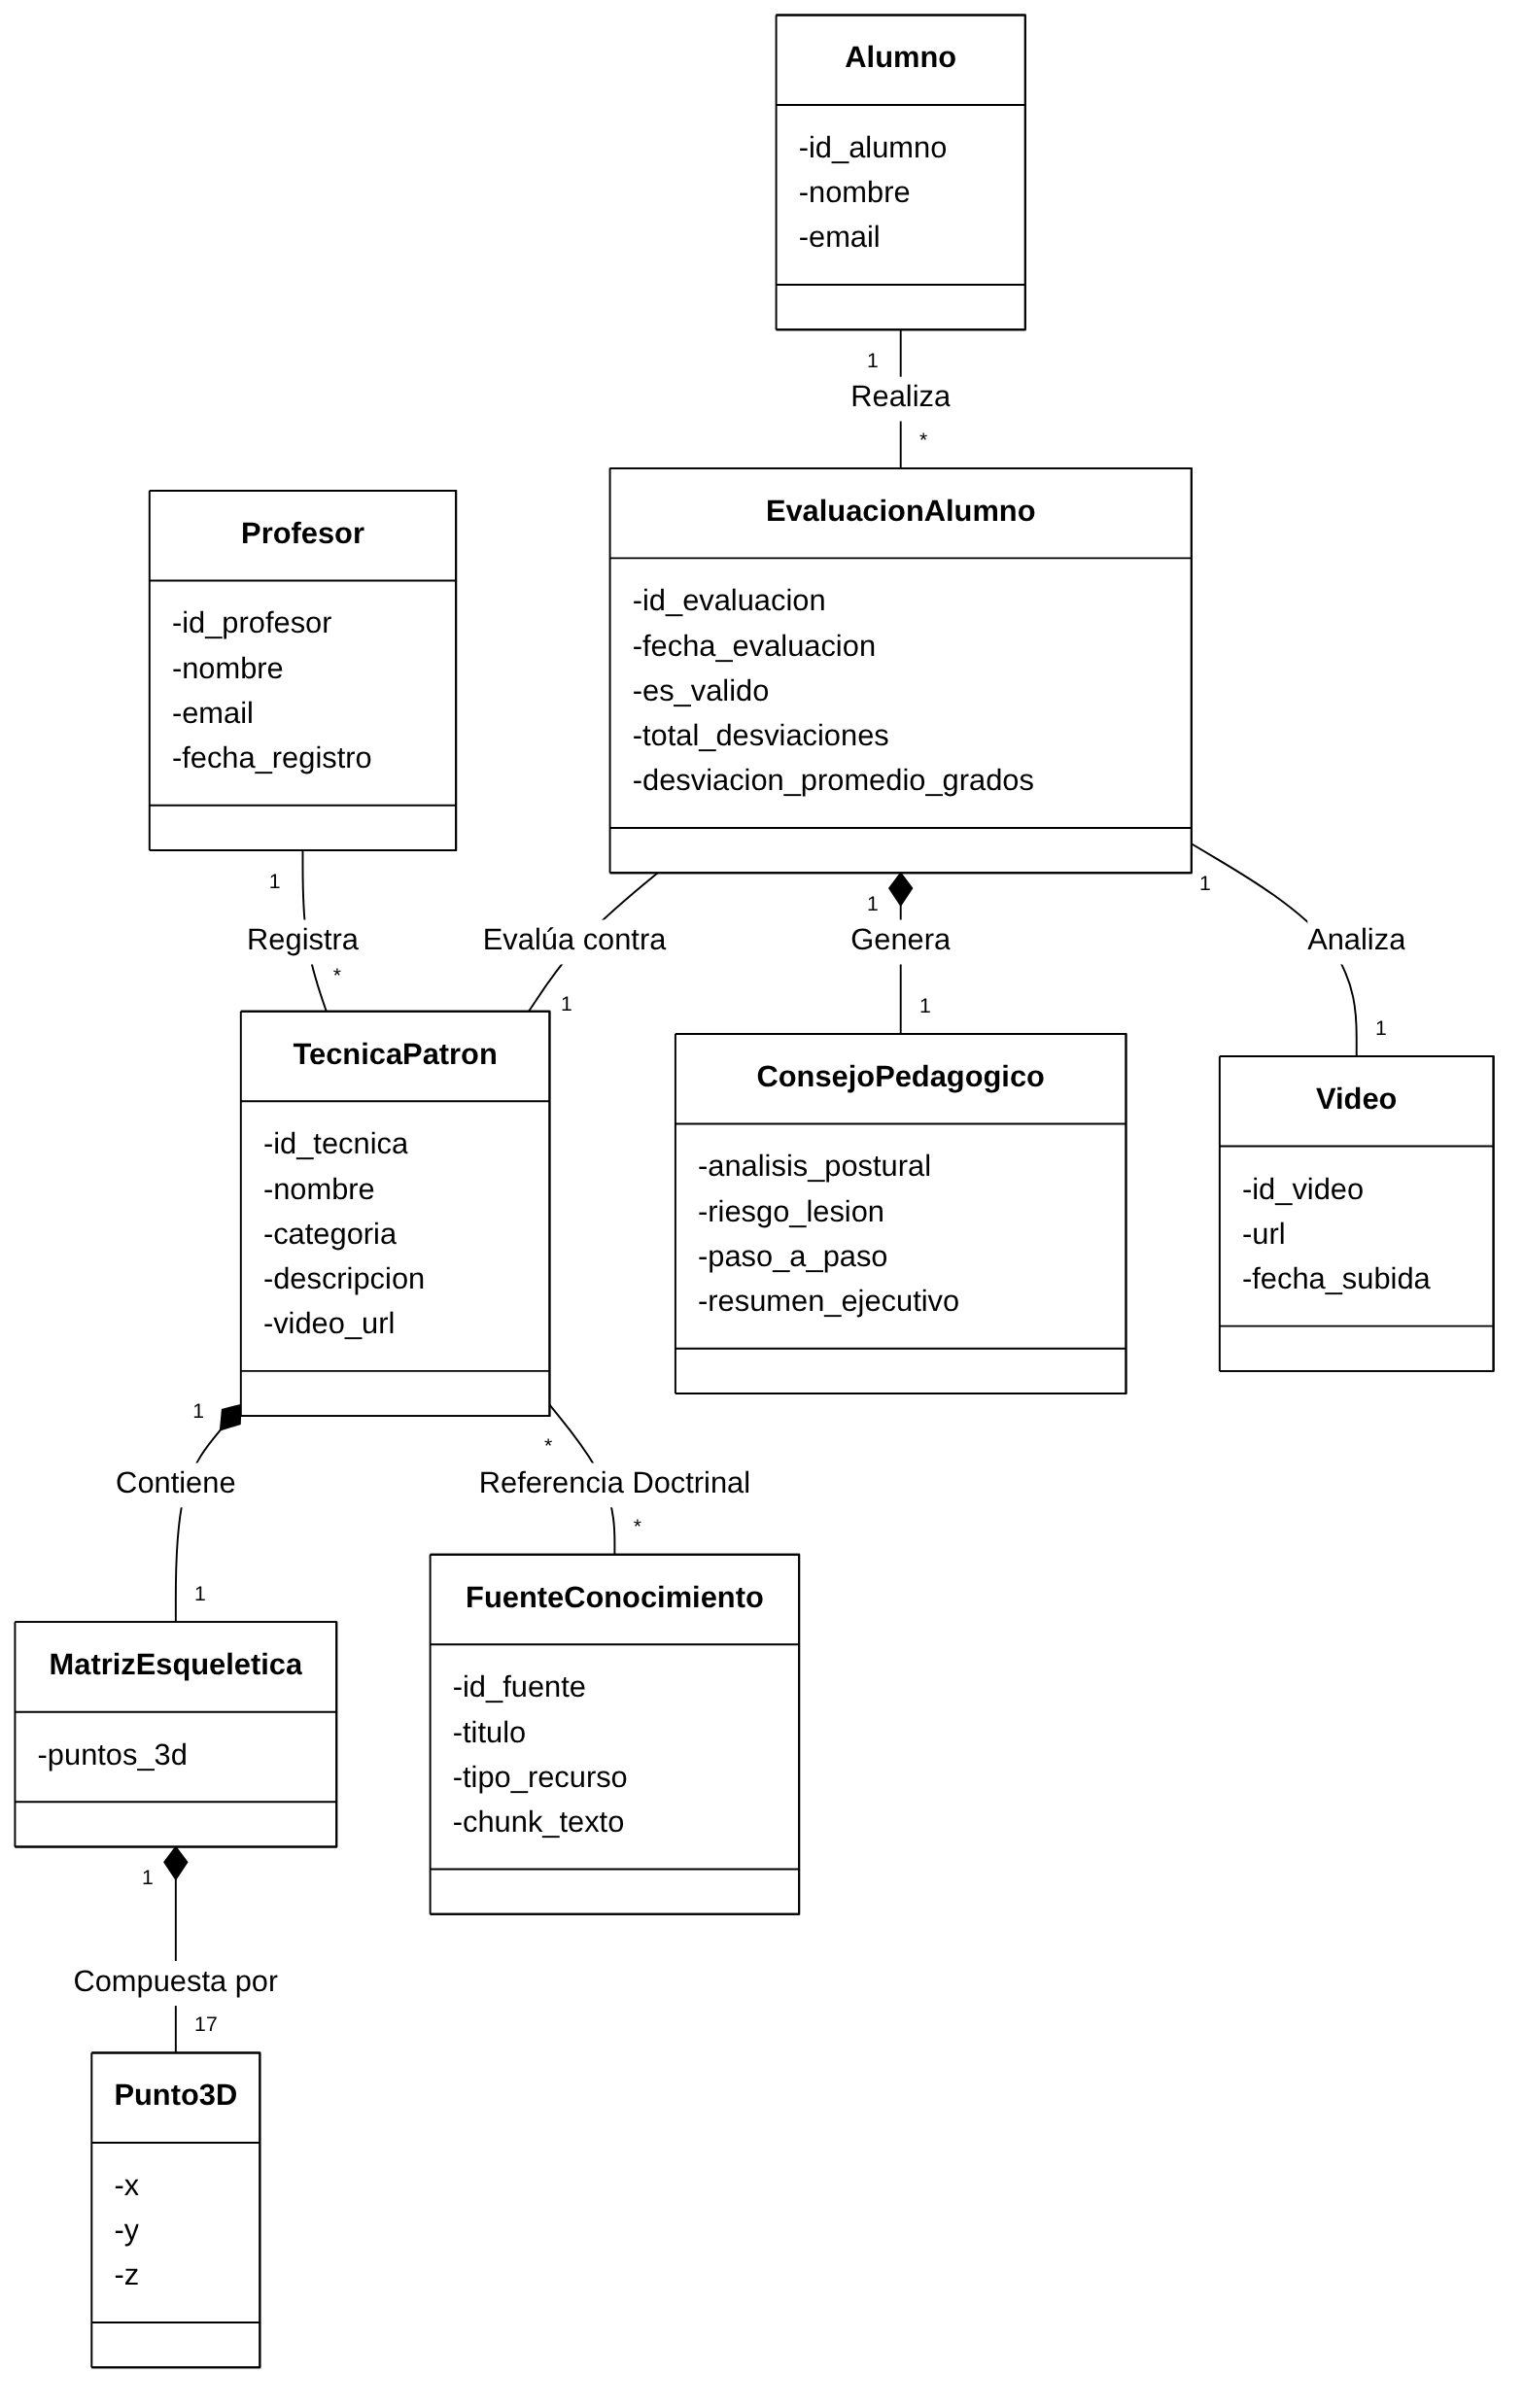
\includegraphics[width=0.9\textwidth,height=0.65\textheight,keepaspectratio]{Figuras/Dominio.png}
    \caption{Modelo de Dominio del Sistema de Análisis Biomecánico BJJ. Fuente: Elaboración propia basada en Larman (2004).}
    \label{fig:modelo-dominio}
\end{figure}

Como se observa en la Figura \ref{fig:modelo-dominio}, el núcleo del dominio se centra en la entidad \texttt{EvaluacionAlumno}, la cual actúa como el vínculo entre el \texttt{Alumno} que realiza la práctica y la \texttt{TecnicaPatron} registrada por el \texttt{Profesor}. La \texttt{MatrizEsqueletica} se compone de 17 objetos \texttt{Punto3D} (keypoints COCO), reflejando la estructura tridimensional extraída por YOLO26x. Además, el \texttt{ConsejoPedagogico} se modela como una entidad dependiente de la evaluación, encapsulando los cuatro bloques de retroalimentación generados por Gemini 2.5 Flash. Las \texttt{FuenteConocimiento} representan los manuales doctrinales que alimentan el motor RAG, estableciendo una relación de referencia doctrinal con las técnicas evaluadas.

\section{Diagramas de Secuencia de Sistema (SSD)}
\label{sec:ssd}

Siguiendo la metodología de Craig Larman (2004), un Diagrama de Secuencia de Sistema (SSD) ilustra el comportamiento de un sistema como una caja negra, mostrando los eventos externos que los actores generan hacia el sistema. Este artefacto es fundamental para identificar las operaciones del sistema que la API REST debe exponer.

\subsection{SSD para el Caso de Uso CU-02: Evaluar Ejecución Biomecánica}
\label{subsec:ssd-cu02}

La Figura \ref{fig:ssd-cu02} presenta el SSD para el escenario principal del caso de uso CU-02. El Alumno interactúa con el Sistema mediante cinco eventos principales: autenticación, selección de técnica, carga de video, consulta de estado y obtención del reporte pedagógico. Nótese que el Sistema se representa como una caja negra (\texttt{:System}), sin revelar los componentes internos que procesan la solicitud, en estricto apego al principio de abstracción de Larman.

\begin{figure}[H]
    \centering
    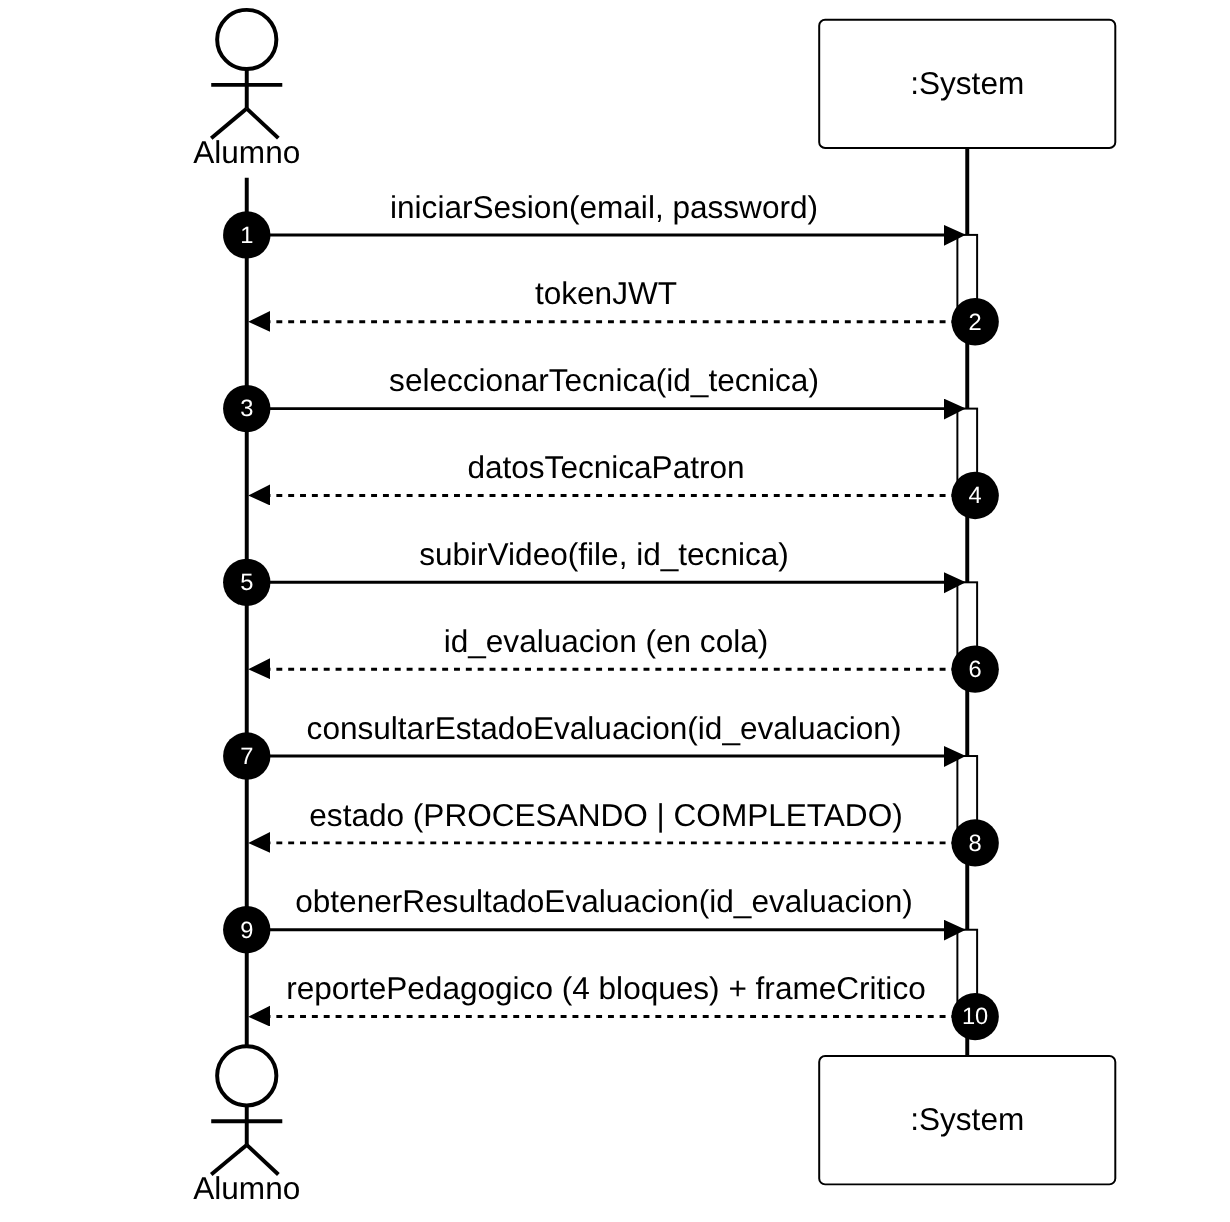
\includegraphics[width=0.9\textwidth]{Figuras/SSD_CU02.png}
    \caption{Diagrama de Secuencia de Sistema (SSD) para el CU-02: Evaluar Ejecución Biomecánica. Fuente: Elaboración propia basada en Larman (2004).}
    \label{fig:ssd-cu02}
\end{figure}

Como se observa en la Figura \ref{fig:ssd-cu02}, los eventos del sistema identificados (\texttt{subirVideo}, \texttt{consultarEstadoEvaluacion}, \texttt{obtenerResultadoEvaluacion}) se convertirán en las operaciones del sistema que se detallarán en los Contratos de Operación. Estos eventos también servirán como punto de partida para los Diagramas de Interacción de diseño.

\subsection{SSD para el Caso de Uso CU-04: Panel de Analítica}
\label{subsec:ssd-cu04}

La Figura \ref{fig:ssd-cu04} presenta el SSD para el CU-04, donde el Instructor solicita las métricas y el sistema retorna el análisis grupal.

\begin{figure}[H]
    \centering
    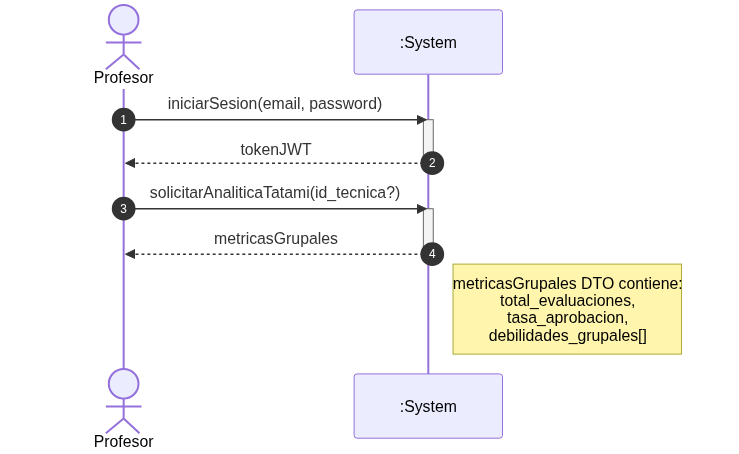
\includegraphics[width=0.8\textwidth]{Figuras/SSD_CU04.png}
    \caption{SSD para CU-04: Panel de Analítica. Fuente: Elaboración propia.}
    \label{fig:ssd-cu04}
\end{figure}

\section{Contratos de Operación}
\label{sec:contratos}

Siguiendo la metodología de Craig Larman (2004, Cap. 13), los Contratos de Operación especifican el comportamiento de las operaciones del sistema en términos de precondiciones y postcondiciones, sin detallar cómo se implementan. Estos contratos se derivan directamente de los SSDs y son un insumo fundamental para el diseño de los Diagramas de Interacción.

\subsection{Contrato CO-01: subirVideo}
\label{subsec:contrato-subir-video}

\begin{table}[H]
\centering
\small
\begin{tabular}{|p{3cm}|p{11cm}|}
\hline
\textbf{Operación} & \texttt{subirVideo(file: Video, id\_tecnica: String)} \\
\hline
\textbf{Referencias} & CU-02: Evaluar Ejecución Biomecánica \\
\hline
\textbf{Precondiciones} & \begin{itemize}
    \item El Alumno está autenticado en el sistema.
    \item La \texttt{TecnicaPatron} con el \texttt{id\_tecnica} especificado existe en el catálogo.
    \item El video cumple con los formatos permitidos (MP4/WebM) y no excede los 50 MB.
\end{itemize} \\
\hline
\textbf{Postcondiciones} & \begin{itemize}
    \item Se creó una instancia \texttt{ev} de \texttt{EvaluacionAlumno} (creación de instancia).
    \item \texttt{ev} se asoció con el \texttt{Alumno} (asociación formada).
    \item \texttt{ev} se asoció con la \texttt{TecnicaPatron} (asociación formada).
    \item \texttt{ev} se asoció con un \texttt{Video} (asociación formada).
    \item El atributo \texttt{estado} de \texttt{ev} se inicializó en "PROCESANDO" (modificación de atributo).
    \item Se asignó un \texttt{id\_evaluacion} único a \texttt{ev} (modificación de atributo).
\end{itemize} \\
\hline
\end{tabular}
\caption{Contrato de Operación CO-01: subirVideo.}
\label{tab:contrato-subir-video}
\end{table}

\subsection{Contrato CO-02: obtenerResultadoEvaluacion}
\label{subsec:contrato-obtener-resultado}

\begin{table}[H]
\centering
\small
\begin{tabular}{|p{3cm}|p{11cm}|}
\hline
\textbf{Operación} & \texttt{obtenerResultadoEvaluacion(id\_evaluacion: String)} \\
\hline
\textbf{Referencias} & CU-02: Evaluar Ejecución Biomecánica \\
\hline
\textbf{Precondiciones} & \begin{itemize}
    \item El Alumno está autenticado en el sistema.
    \item Existe una \texttt{EvaluacionAlumno} con el \texttt{id\_evaluacion} especificado.
    \item El estado de la \texttt{EvaluacionAlumno} es "COMPLETADO".
\end{itemize} \\
\hline
\textbf{Postcondiciones} & \begin{itemize}
    \item Se recuperó la instancia \texttt{ev} de \texttt{EvaluacionAlumno} (consulta de instancia).
    \item Se recuperó el \texttt{ConsejoPedagogico} asociado a \texttt{ev} (consulta de asociación).
    \item Se recuperó la \texttt{TecnicaPatron} asociada a \texttt{ev} (consulta de asociación).
    \item Se recuperó el \texttt{Video} y el \texttt{frameCritico} asociado a \texttt{ev} (consulta de asociación).
\end{itemize} \\
\hline
\end{tabular}
\caption{Contrato de Operación CO-02: obtenerResultadoEvaluacion.}
\label{tab:contrato-obtener-resultado}
\end{table}

\subsection{Contrato CO-03: obtenerDebilidadesGrupales}
\label{subsec:contrato-co03}

\textbf{Operación:} \texttt{obtenerDebilidadesGrupales(id\_tecnica)} \\
\textbf{Referencias Cruzadas:} Casos de Uso: CU-04. \\
\textbf{Precondiciones:} 
\begin{itemize}
    \item Existe un historial de evaluaciones almacenadas en el sistema.
\end{itemize}
\textbf{Postcondiciones:} 
\begin{itemize}
    \item Se han calculado las frecuencias y promedios de desviación por articulación.
    \item Se ha devuelto un resumen estadístico ordenado por mayor frecuencia de error.
\end{itemize}

\section{Diagramas de Interacción (Realizaciones de Casos de Uso)}
\label{sec:interaccion}

Siguiendo la metodología de Craig Larman (2004, Cap. 16-17), un Diagrama de Interacción (también llamado Realización de Caso de Uso) muestra cómo los objetos de software colaboran para llevar a cabo el comportamiento especificado en un caso de uso. Estos diagramas aplican los patrones GRASP (Controller, Expert, Creator, Low Coupling, Protected Variations) para asignar responsabilidades a los objetos.

\subsection{Realización del CU-02: Evaluar Ejecución Biomecánica}
\label{subsec:interaccion-cu02}

La Figura \ref{fig:interaccion-cu02} presenta el diagrama de interacción para el escenario principal del caso de uso CU-02. El \texttt{EvaluacionController} actúa como un Controlador (GRASP Controller) que delega las responsabilidades a los objetos expertos:
\begin{itemize}
    \item \texttt{AdaptadorYOLO} se encarga de la inferencia de visión artificial (Protected Variations).
    \item \texttt{PostgresTecnicaRepository} recupera el patrón esquelético (Expert).
    \item \texttt{CalculadoraBiomecanica} computa las desviaciones angulares (Expert / Pure Fabrication).
    \item \texttt{SintesisPedagogicaService} orquesta la búsqueda RAG (Pure Fabrication).
    \item \texttt{QdrantAdapter} y \texttt{GeminiServiceAdapter} son adaptadores de infraestructura (Protected Variations).
\end{itemize}

\begin{figure}[H]
    \centering
    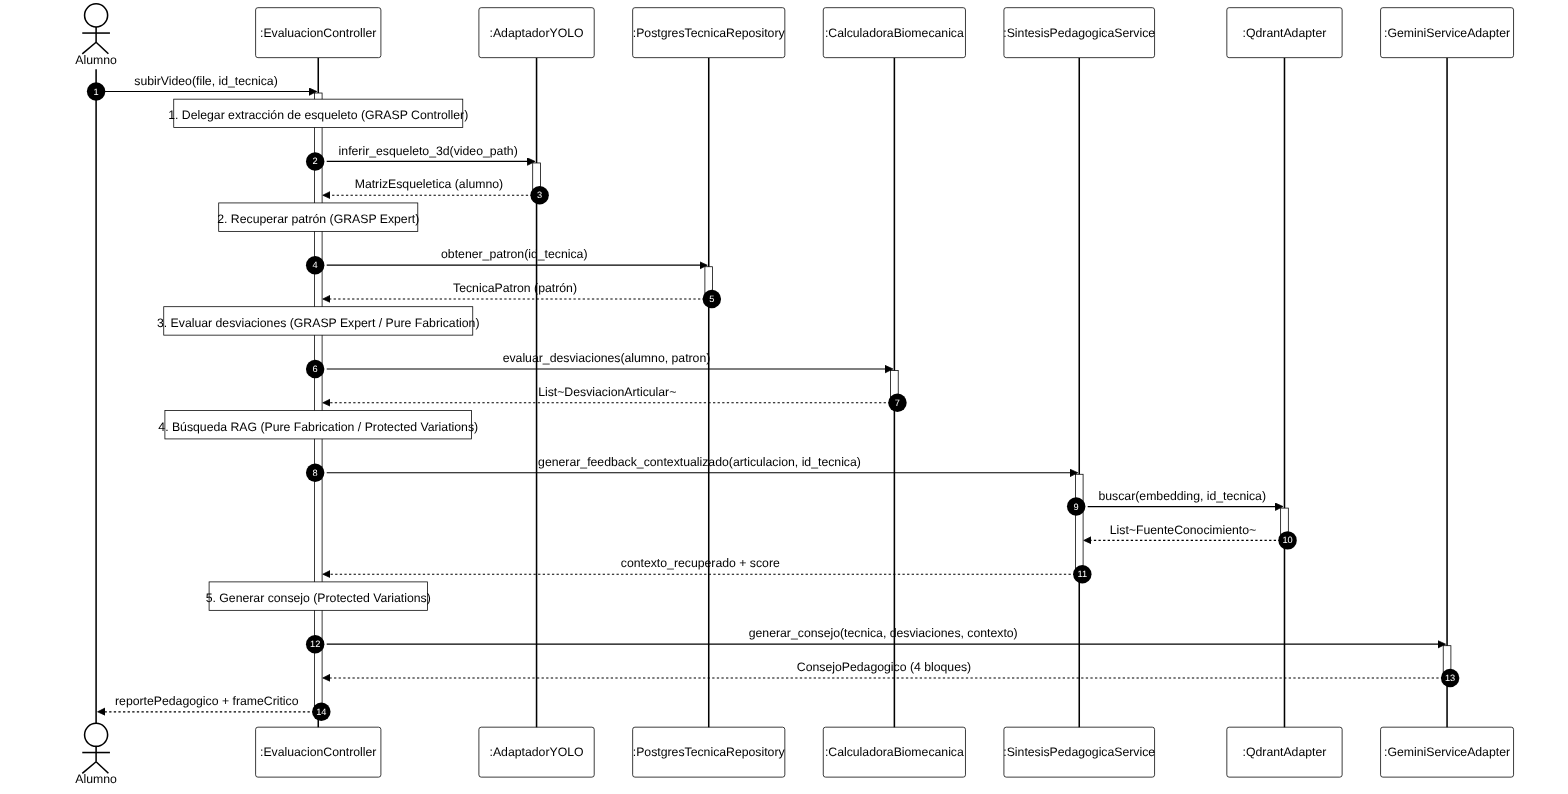
\includegraphics[width=1.0\textwidth]{Figuras/Interaccion_CU02.png}
    \caption{Diagrama de Interacción (Realización de Caso de Uso) para el CU-02: Evaluar Ejecución Biomecánica. Fuente: Elaboración propia basada en Larman (2004).}
    \label{fig:interaccion-cu02}
\end{figure}
Como se observa en la Figura \ref{fig:interaccion-cu02}, la secuencia de mensajes refleja fielmente los Contratos de Operación (Sección 5.3) y prepara el terreno para el Diagrama de Clases de Diseño (Sección 5.5), donde se detallarán los atributos, métodos y relaciones entre estas clases.

\subsection{Realización del CU-04: Panel de Analítica}
\label{subsec:realizacion-cu04}

La interacción principal para el CU-04 implica que la UI solicita datos al \texttt{AnaliticaController}, el cual obtiene el historial completo del \texttt{IHistorialRepository} y calcula las métricas en memoria.

\section{Diagrama de Clases de Diseño (DCD)}
\label{sec:dcd}

Siguiendo la metodología de Craig Larman (2004, Cap. 19), el Diagrama de Clases de Diseño (DCD) consolida las decisiones estáticas tomadas durante el diseño de las interacciones. Mientras que el Modelo de Dominio (Sección 5.1) representa conceptos del mundo real, el DCD muestra las clases de software reales que participan en la solución, con sus atributos tipados, métodos y relaciones de navegabilidad.

\subsection{DCD para el CU-02: Evaluar Ejecución Biomecánica}
\label{subsec:dcd-cu02}

La Figura \ref{fig:dcd-cu02} presenta el Diagrama de Clases de Diseño para el CU-02. Este diagrama refleja la separación de capas y la aplicación de los patrones GRASP:
\begin{itemize}
    \item \texttt{EvaluacionController} (Capa de Aplicación) actúa como Session Facade (GRASP Controller).
    \item \texttt{CalculadoraBiomecanica}, \texttt{MatrizEsqueletica}, \texttt{Punto3D} y \texttt{DesviacionArticular} (Capa de Dominio) aplican Expert y Pure Fabrication.
    \item \texttt{AdaptadorYOLO}, \texttt{GeminiServiceAdapter}, \texttt{QdrantAdapter} y \texttt{PostgresTecnicaRepository} (Capa de Infraestructura) implementan las interfaces de dominio aplicando Protected Variations.
    \item \texttt{SintesisPedagogicaService} (Capa de Servicios) es una Pure Fabrication que orquesta el RAG.
\end{itemize}

\begin{figure}[H]
    \centering
    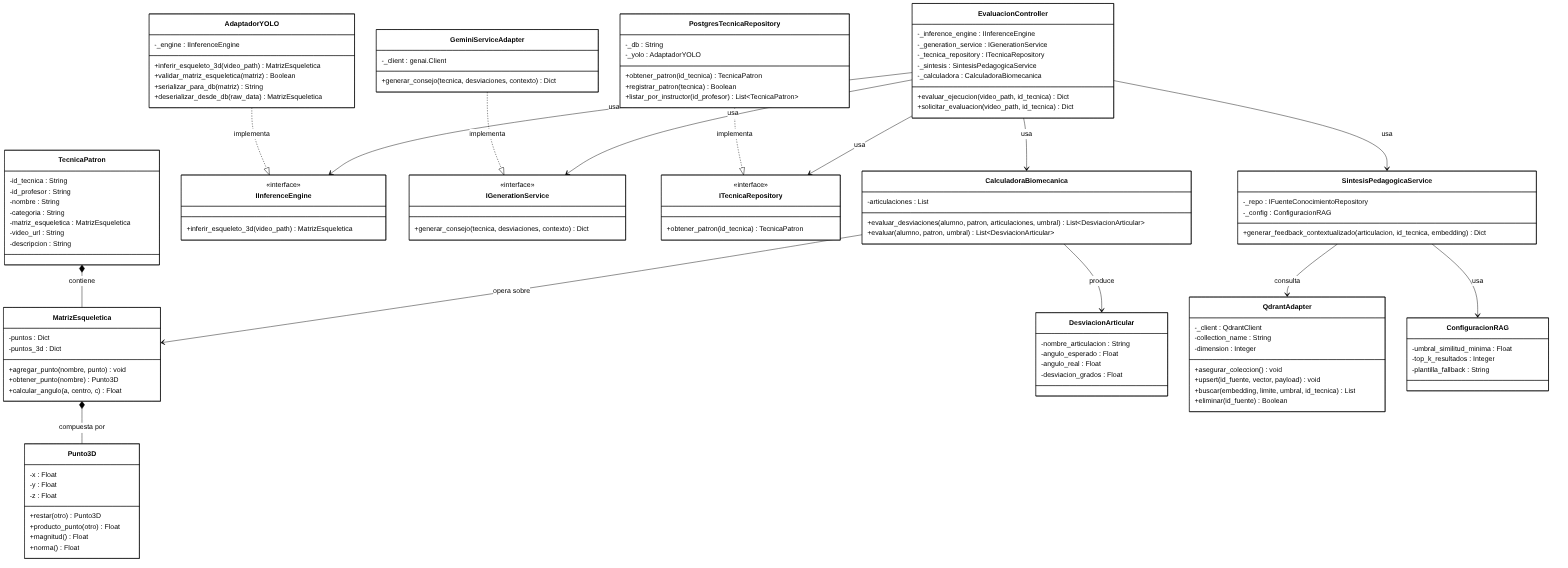
\includegraphics[width=1.0\textwidth]{Figuras/DCD_CU02.png}
    \caption{Diagrama de Clases de Diseño (DCD) para el CU-02: Evaluar Ejecución Biomecánica. Fuente: Elaboración propia basada en Larman (2004).}
    \label{fig:dcd-cu02}
\end{figure}

Como se observa en la Figura \ref{fig:dcd-cu02}, el DCD evidencia la correcta aplicación de los patrones GRASP y la arquitectura en capas del sistema, garantizando bajo acoplamiento y alta cohesión. Las interfaces (\texttt{IInferenceEngine}, \texttt{IGenerationService}, \texttt{ITecnicaRepository}) permiten que la capa de aplicación sea agnóstica a los detalles de implementación, facilitando la sustitución de adaptadores sin afectar la lógica de negocio (Protected Variations).
Como se observa en la Figura \ref{fig:dcd-cu02}, el DCD evidencia la correcta aplicación de los patrones GRASP y la arquitectura en capas del sistema, garantizando bajo acoplamiento y alta cohesión. Las interfaces (\texttt{IInferenceEngine}, \texttt{IGenerationService}, \texttt{ITecnicaRepository}) permiten que la capa de aplicación sea agnóstica a los detalles de implementación, facilitando la sustitución de adaptadores sin afectar la lógica de negocio (Protected Variations).

\subsection{DCD para el CU-04: Panel de Analítica}
\label{subsec:dcd-cu04}

La Figura \ref{fig:dcd-analitica} muestra el DCD que incorpora el \texttt{AnaliticaController} y la actualización del \texttt{IHistorialRepository} para soportar la agregación de métricas.

\begin{figure}[H]
    \centering
    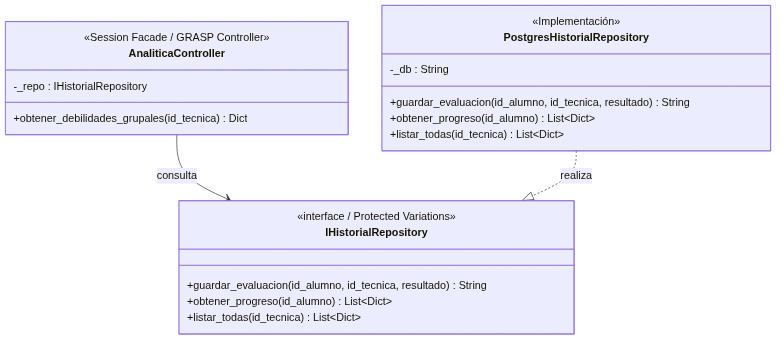
\includegraphics[width=1.0\textwidth]{Figuras/DCD_Analitica.png}
    \caption{DCD para CU-04. Fuente: Elaboración propia.}
    \label{fig:dcd-analitica}
\end{figure}

\section{Software Architecture Document (SAD)}
\label{sec:sad}

Siguiendo la metodología de Craig Larman (2004, Cap. 32), el Software Architecture Document (SAD) es un artefacto que consolida las decisiones arquitectónicas, las vistas de arquitectura y los factores que influyen en el diseño del sistema. Este documento sirve como una guía de aprendizaje para desarrolladores futuros y como evidencia de la correcta aplicación de los patrones arquitectónicos.

\subsection{Vista Lógica (Logical View)}
\label{subsec:vista-logica}

La Vista Lógica describe la organización conceptual del software en capas, paquetes y subsistemas. El sistema BJJ Biomechanics se organiza en 5 capas siguiendo el patrón \textit{Layers} de Larman:

\begin{itemize}
    \item \textbf{Presentation Layer}: PWA (HTML/JS/CSS) y API REST FastAPI.
    \item \textbf{Application Layer}: Controladores (Session Facades) que orquestan los casos de uso.
    \item \textbf{Services Layer}: Pure Fabrications (Chunker, SintesisPedagogicaService).
    \item \textbf{Domain Layer}: Entidades puras (MatrizEsqueletica, CalculadoraBiomecanica, Punto3D).
    \item \textbf{Infrastructure Layer}: Adaptadores (YOLO, Gemini, Qwen, Qdrant) y Repositorios PostgreSQL.
\end{itemize}

La Figura \ref{fig:arquitectura-capas} ilustra la organización de las capas y sus dependencias.

\begin{figure}[H]
    \centering
    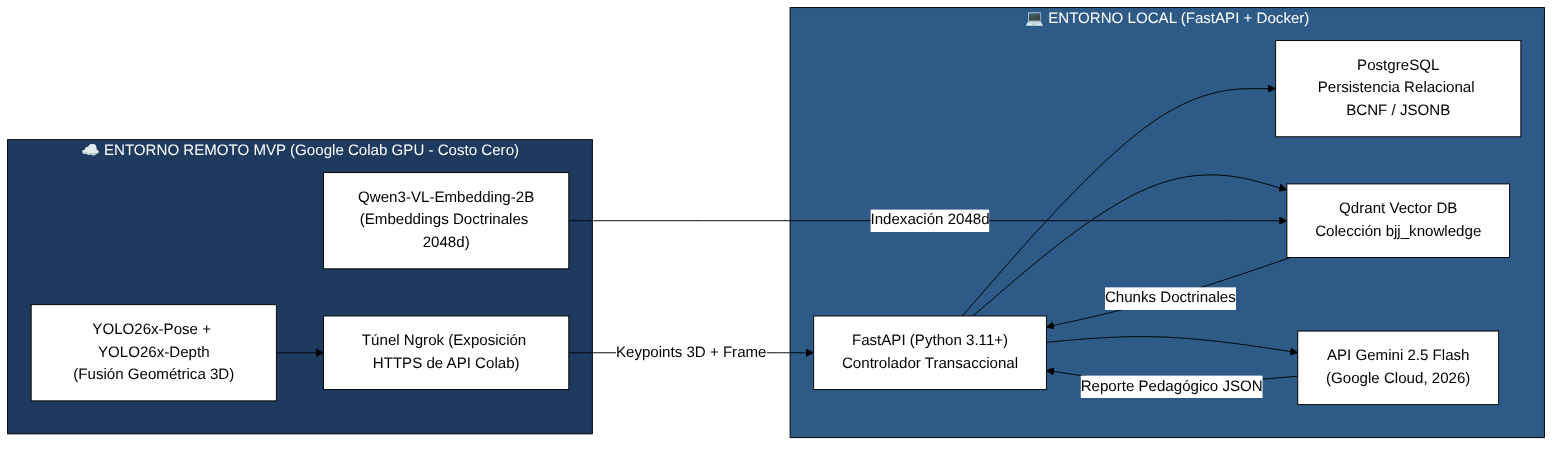
\includegraphics[width=1.0\textwidth]{Figuras/Arquitectura.png}
    \caption{Vista Lógica de la Arquitectura: Patrón Layers. Fuente: Elaboración propia basada en Larman (2004).}
    \label{fig:arquitectura-capas}
\end{figure}

\subsection{Vista de Procesos (Process View)}
\label{subsec:vista-procesos}

La Vista de Procesos describe los procesos, hilos y la comunicación entre ellos. En el sistema BJJ Biomechanics, los procesos principales son:

\begin{itemize}
    \item \textbf{Proceso Local (FastAPI + Uvicorn)}: Ejecuta la API REST, los controladores y la lógica de dominio. Se comunica con PostgreSQL y Qdrant.
    \item \textbf{Proceso Remoto (Google Colab GPU)}: Ejecuta la inferencia de YOLO26x-Pose + YOLO26x-Depth. Se comunica con el proceso local mediante túnel Ngrok (HTTPS).
    \item \textbf{Proceso Externo (Gemini API)}: Ejecuta la síntesis pedagógica. Se comunica con el proceso local mediante HTTPS.
\end{itemize}

\subsection{Vista de Despliegue (Deployment View)}
\label{subsec:vista-despliegue}

La Vista de Despliegue describe la asignación de procesos a nodos de procesamiento. La Figura \ref{fig:despliegue} presenta la topología de despliegue del sistema.

\begin{figure}[H]
    \centering
    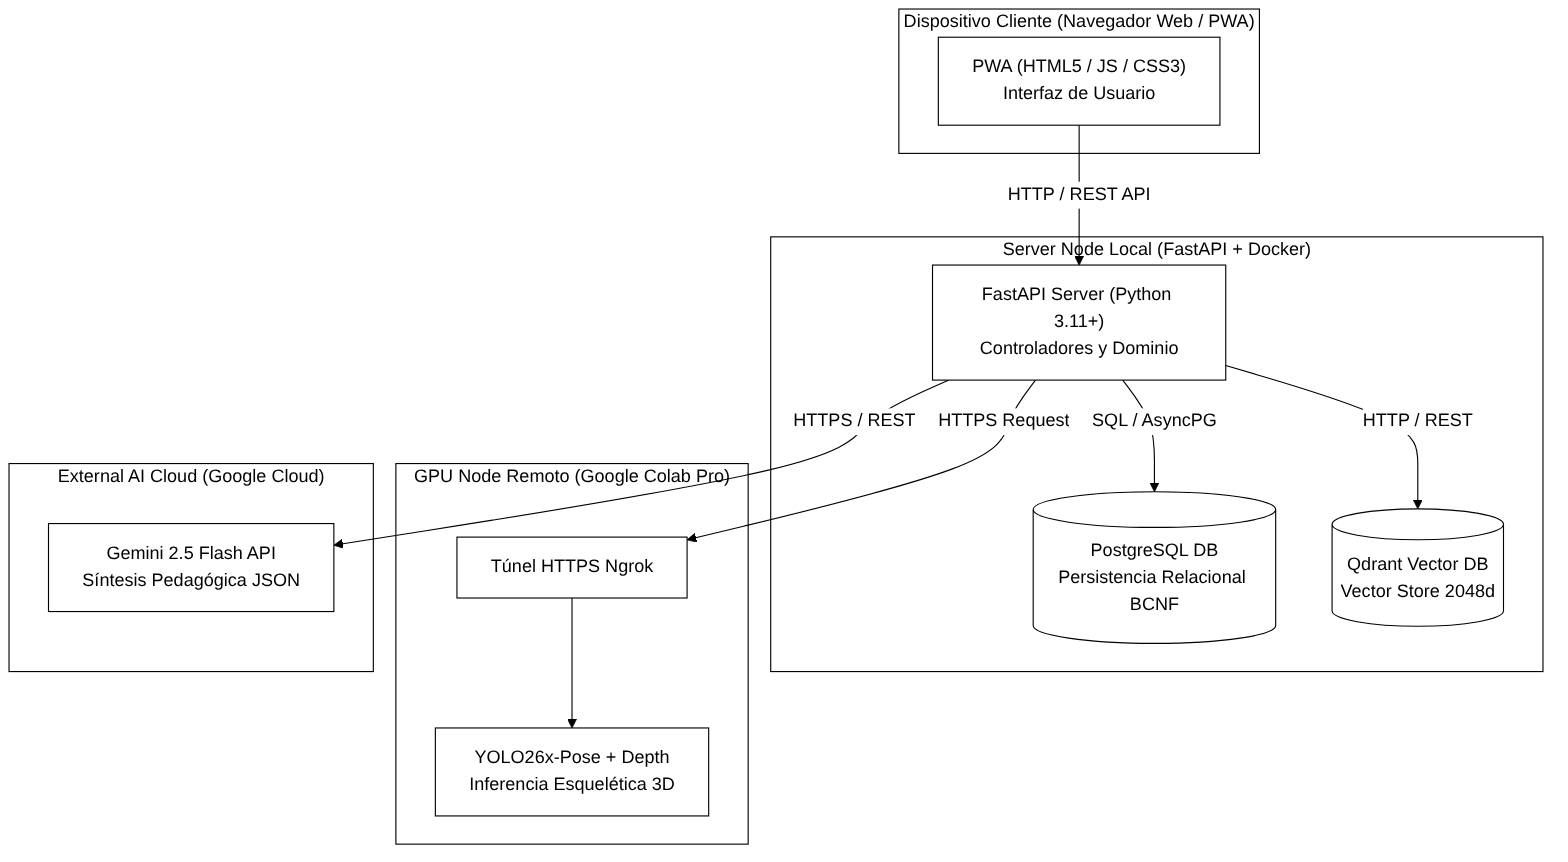
\includegraphics[width=1.0\textwidth]{Figuras/Despliegue.png}
    \caption{Vista de Despliegue: Topología de Nodos y Túnel Ngrok. Fuente: Elaboración propia basada en Larman (2004).}
    \label{fig:despliegue}
\end{figure}

\subsection{Vista de Datos (Data View)}
\label{subsec:vista-datos}

La Vista de Datos describe el esquema de persistencia. El sistema utiliza una arquitectura híbrida:

\begin{itemize}
    \item \textbf{PostgreSQL (BCNF)}: Almacena metadatos relacionales (usuarios, profesores, técnicas, evaluaciones, fuentes). La columna JSONB \texttt{consejo\_pedagogico} almacena el reporte estructurado de 4 claves.
    \item \textbf{Qdrant (Vector Store)}: Almacena los embeddings de 2048 dimensiones de los manuales doctrinales, con metadatos relacionales (id\_tecnica, id\_documento) para filtrado semántico.
\end{itemize}

\subsection{Technical Memos: Decisiones Arquitectónicas Clave}
\label{subsec:technical-memos}

A continuación se presentan las decisiones arquitectónicas más relevantes, documentadas según el formato de Technical Memos de Larman (Cap. 32).

\subsubsection{Technical Memo 1: Uso de Qdrant en lugar de pgvector}

\textbf{Problema}: pgvector limita los índices HNSW/IVFFlat a un máximo de 2000 dimensiones. Qwen3-VL-Embedding-2B produce vectores de 2048 dimensiones.

\textbf{Solución}: Se seleccionó Qdrant como base de datos vectorial especializada, ejecutada on-premise vía Docker.

\textbf{Motivación}: Qdrant permite indexación eficiente con filtros de metadatos (id\_tecnica, id\_documento) sin restricciones de dimensionalidad, garantizando soberanía de datos y costo cero operativo.

\subsubsection{Technical Memo 2: Uso de Google Colab GPU + Ngrok}

\textbf{Problema}: La inferencia sincrónica de YOLO26x-Pose + YOLO26x-Depth requiere aceleración GPU intensiva. Los servidores locales con GPU tienen costos fijos elevados.

\textbf{Solución}: Se delegó la inferencia a Google Colab Pro (GPU NVIDIA T4/A100), comunicado mediante túnel Ngrok.

\textbf{Motivación}: Esta arquitectura desacoplada permite ejecutar el análisis pesado en servidores remotos sin costo de infraestructura durante la fase de MVP, siguiendo el patrón Adapter para proteger el núcleo del sistema.

\subsubsection{Technical Memo 3: Uso de Gemini 2.5 Flash para Síntesis Estructurada}

\textbf{Problema}: Se requiere generar reportes pedagógicos estructurados en JSON con 4 claves obligatorias (Análisis Postural, Riesgo de Lesión, Paso a Paso, Resumen Ejecutivo).
\textbf{Solución}: Se seleccionó Gemini 2.5 Flash por su soporte nativo para forzar respuestas bajo esquemas JSON estrictamente estructurados y su excelente relación velocidad/costo.

\end{document}

\subsubsection{Technical Memo 4: Agregación de Métricas en Memoria vs. Base de Datos}
\textbf{Problema:} ¿Dónde deben calcularse las estadísticas de debilidades (CU-04)? \\
\textbf{Solución:} Se optó por extraer todas las evaluaciones y calcular los promedios en memoria dentro del \texttt{AnaliticaController}. \\
\textbf{Justificación (Patrones GRASP/SOLID):} Debido a la estructura de esquemas JSON estrictamente estructurados dentro de PostgreSQL y la necesidad de compatibilidad retroactiva, la lógica compleja en SQL (o \texttt{jsonb\_path\_query}) resultaba frágil. Siguiendo el principio de \textit{Protected Variations}, la base de datos se mantiene simple y la lógica de agregación reside en Python, permitiendo escalar a repositorios NoSQL o archivos estáticos en el futuro sin modificar la lógica de cálculo.
